%\documentclass[a4paper, english,10pt]{article}
%\documentclass[english,10pt, oneside, draft, a4paper]{report}
%\documentclass[english,10pt, oneside, a4paper]{scrreprt}
%\usepackage[b5paper, layout=b5paper, textwidth=12cm, twoside,bindingoffset=1cm,outer=2cm,inner=2cm,includefoot,bmargin=3cm]{geometry}
%\usepackage[a4paper, layout=a4paper, textwidth=12cm, bindingoffset=1cm,outer=2cm,inner=2cm,includefoot,bmargin=3cm]{geometry}
\documentclass[english,10pt, twoside, b5paper]{book}%scrreprt
\usepackage[lmargin=20mm,rmargin=20mm,tmargin=25mm,bmargin=35mm,bindingoffset=1cm,textwidth=12cm,includefoot,includehead]{geometry}


\RequirePackage[l2tabu, orthodox]{nag}
\usepackage{lmodern}
\usepackage[english]{babel}
\usepackage[utf8]{inputenc}
\usepackage[T1]{fontenc}
\usepackage{float}
\usepackage{subcaption}
\usepackage{multirow}
\usepackage{tabularx}
\usepackage{perpage} % For å få fotnotenummerering til å starte på nytt for hver side
\usepackage{graphicx}
\graphicspath{{grafikk/}}
\usepackage[export]{adjustbox} %In including a figure, add "center" as a flag

\usepackage{makecell}
\usepackage{epstopdf}
\usepackage{varioref}
\usepackage{listings} % For å vise frem kode på en bra måte
\usepackage{textgreek}
%\usepackage{tikz,pgfplots} % For å plotte Matlab figurer på en god måte
\usepackage{amsmath} % For å tilpasse ligninger til å vises over flere linjer
\usepackage{pdfpages} % For å legge til pdf i appendix delen
\usepackage{rotating}
\usepackage{hyperref} % [pdfborder=0]{hyperref} to remove borders around
% pdf-links.
%\usepackage[text={6.2in,9.5in},centering]{geometry}
\usepackage{mathtools}
\usepackage{color} % Farger i dokumentet

\usepackage{dialogue}
\usepackage[section]{placeins}
\usepackage{microtype}

\linespread{1.5}

% \lstset{frame=shadowbox, rulesepcolor=\color{black}}
\lstset{numbers=left, frame=single, tabsize=2, breaklines=true}

\DeclarePairedDelimiter\abs{\lvert}{\rvert}%
\DeclarePairedDelimiter\norm{\lVert}{\rVert}%

\makeatletter
\let\oldabs\abs
\def\abs{\@ifstar{\oldabs}{\oldabs*}}
%
\let\oldnorm\norm
\def\norm{\@ifstar{\oldnorm}{\oldnorm*}}
\makeatother


\DeclareMathSymbol{\comma}{\mathpunct}{letters}{"3B} % Legger inn kommandoen \comma som komma i math mode

\hypersetup{%
    pdfborder = {0 0 0}
}

%\usepackage{endnotes}
%\usepackage[portrait, pdftex]{geometry}

\newcommand{\HRule}{\rule{\linewidth}{0.5mm}}
\pretolerance = 1414
\tolerance = 1414

\MakePerPage{footnote} % For å få fotnotenummerering til å starte på nytt for hver side
\labelformat{equation}{equation~(#1)}
\labelformat{figure}{figure~{#1}}
\labelformat{subfigure}{figure~\thefigure #1}
\labelformat{table}{table~{#1}}
\labelformat{section}{section~{#1}}
\labelformat{subsection}{section~{#1}}
\labelformat{chapter}{chapter~{#1}}


% ########################################## 
%			Beginning of document
% ########################################## 

\begin{document}

\setcounter{tocdepth}{5}
\setcounter{secnumdepth}{5}

\setcounter{page}{0}
\pagenumbering{roman}
% \pagedial{empty}

%Does the report contain the necessary elements as 
%abstract/summary, 
%table of 
%contents, 
%introduction, etc. in an appropriate form 

%starting point/objectives, 
%what is done and the 
%conclusions/results, and to maintain this overview throughout the reading. 

% #### Other stuff from the template

%\title{Piloting map service for navigating in punctuality analysis for trains \\ \vspace{2 mm} {\large A case study of railway
%operations}}\date{ June 17, 2014}


%\begin{titlepage}
%\begin{center}

%\vspace{10mm}
%
\includegraphics[width=0.55\textwidth]{logo_ntnu_eng.png}~\\[1cm]
% \vspace{30mm}

%\makeatletter
%    \parindent \z@
%    \reset@font
%    \vskip 40\p@
%    \par
%    \hrule height 2pt
%    \par
%    \vskip 4\p@
%    \huge \@title
%    \vskip 6\p@
%    \par
%    \hrule height 2pt
%    \par
%    \begin{flushright}
%      \large \@date \par
%    \end{flushright}
%    \vskip 100\p@
% \vspace{20mm}
%\begin{minipage}{0.4\textwidth}
%\begin{flushleft} \large
%\centerline{Magnus Krane}
%~\\
%\centerline{Supervisor:}
%\centerline{Sobah Petersen}
%\centerline{Co-supervisor:}
%\centerline{Andreas Dypvik Landmark - SINTEF}
%\end{flushleft}
%\end{minipage}
%\vfill
%\end{center}
%\end{titlepage}

\section*{Problem Description} % (fold)
\label{sec:_problem_description}

% section _problem_description (end)

\subsection*{Piloting map service for navigating in punctuality analysis for 
trains}

Conceptualize and develop prototype of map based visualizations of real time signal data to improve punctuality.


\cleardoublepage
\phantomsection
\addcontentsline{toc}{section}{Summary}
\section*{Summary}

		XXX

\clearpage

\cleardoublepage
\phantomsection
\addcontentsline{toc}{section}{Norwegian Abstract}
\section*{Sammendrag (Norwegian Abstract)}

I et komplekst system som det norske jernbane nettverket er det mye som kan
påvirke punkligheten til et tog. Operatørene på jernbanen streber etter å oppnå
høyere og høyere punklighet. Infrastruktur eier, Jernbaneverket,  streber etter
minst mulig nedetid på trafikk nettverket.
Ved å analysere og sammenligne forskjellige data sett er det mulig å forstå grunnen til forsinkelsene.
%Setning for å henge sammen over og under kommentar
Ulike brukere har forskjellig behov når de studerer data settene. For eksempel
så har en direktør behovet for å kunne se hele bildet, mens
strekningsansvarlige har behov for å kunne studere hver minste detalj.\\

I denne masteroppgaven skal demonstrerer vi et system som tar hensyn til de
forskjellige brukerene sine behov for forskjellig presentasjon av data.
Systemet tar også hensyn til behovene for å kunne se på forskjellige data
og sammenligne disse.
	
\clearpage

\cleardoublepage
\phantomsection
\addcontentsline{toc}{section}{Preface}
\section*{Preface}

The work of this thesis has been performed at the Department of Computer and
Information Science (IDI) at the Norwegian University of Science and Technology
(NTNU), and in collaboration with SINTEF Technology and Society during the
spring semester of 2014. \\

During the work of this thesis, I have been supervised by Sobah Abbas Pettersen
and co-supervised by researcher Andreas Landmark (SINTEF), research manager
Andreas Seim (SINTEF), and researcher Rimmert van der Kooij (SINTEF), who have
all been a great help throughout the process, providing valuable input and
guidance.

I would also like to thank fellow students Magnus Bae and Bjørn Thomas Vee for
feedback and help when needed.\\

I have also been part of the student organization Revolve NTNU this semester,
which is a group of students building a prototype formula student race car for
participating in the international Formula Student competitions. I would like
thank my fellow team members for participating in some of the best times I have
experienced.

A final thank you to my supervisors for understanding that participating in
Revolve NTNU has made time difficult to balance.

\mbox{}\\[1pc]
Trondheim, \today\\
\mbox{}\\[1pc]
Magnus Krane

\clearpage

\cleardoublepage

\renewcommand\contentsname{Table of Contents}
\tableofcontents
\cleardoublepage
\renewcommand\listfigurename{List of Figures}
\listoffigures
\cleardoublepage
\renewcommand\listtablename{List of Tables}
\listoftables
\cleardoublepage

%\chapter*{Definitions \& abbreviations}
%%Abbreviations and definitions
\label{sec:abbriv}
\vspace{5mm}

\begin{description}
\item [GIS] Geographic information system
\item [Regularity]	Jernbaneverket defines regularity as the number of trains that gets run as planed in the time schedule. 
\item [Uptime]	Jernbaneverket states that uptime in regards to punctuality defines from hours of delay caused by infrastructure relative to sum of planed train hours per year. \begin{equation} Uptime =
\frac{\text{Train hours - hours of delay}}{\text{Train hours}}\times 100 \end{equation}
\end{description}



\cleardoublepage

\setcounter{page}{0}
\pagenumbering{arabic}


% !TEX root=../thesis.tex

\chapter{Introduction}

In this report we aim to design a software architecture for a driver information
system\footnote{Also known as In Vehicle Information System, IVIS}
that is to be prototyped and installed in a formula student race car. We will
also discuss the state of the art, technological alternatives and introduce
background information pertaining to the domain and use-cases.

To design this architecture we have undertaken a significant literature study
of both architectural design patterns and driver/operator information systems.
We have looked at what a typical driver information system does, how it does
it, and what the state of the art is. Other fields employing information 
systems to provide vehicle operators with real-time information have also been
studied.

This research effort is made to serve as a foundation to build a prototype
driver information system in collaboration with Revolve NTNU (Revolve), a 
student organization  created by students at the Norwegian University of 
Science and Technology.
The the collaboration with Revolve will serve as a testing ground for our 
design and allow us to test its feasibility in the
context of motorsport.

For the last three years Revolve has been hard at work building formula style race
cars to participate in events of the international motor sport competition series
``Formula Student'' (FS). The competitions are arranged by the Institution of Mechanical Engineers. In the competitions teams of students compete against each other
with small formula-style cars they have designed and built from scratch. There are
disciplines that involves racing the cars as well as disciplines in business,
design, and cost. The combined score from these events decide the official
results, but there are also prices awarded for excellence in different fields

Motorsport has for many years been a testbed for car manufacturers and a lot of
technology that we today take for granted has come to fruition through motorsport. However
ordinary cars have seen larger leaps in technology with regards to information
consumption than cars built for motor racing. For some years some high-end cars
have even been equipped with heads-up displays (HUD) that allows the driver to 
keep focus on the road instead of looking down at the instruments \cite{wiki:hud},
and it is becoming more and more common.

Despite great developments in automobile technology over the past 50 years little
has changed in the way that motorsport drivers receives information during an
event. There are displays, gauges, and other visual indicators\footnotemark[1]
, in addition to radio-communication \cite{wiki:formula_radio} if that is allowed in the competition. The technology under the hood
has become much more advanced, but the amount of information you can
convey to the driver still seems to be very limited; the pace is just too high
to be able to keep moving focus from the road (see appendix \vref{interview:bakkom}).

Driver information systems in the context of motorsport is a field neglected by
science (see \vref{background:rel_reasearch}). There has been done some
research around driver information systems in commercial vehicles and normal 
passenger cars, most of which involve studies of heads-up display technology or
use.

This is therefore a field where we are threading into new territory. 
Requirements are hard to elicit up front, and we don't know
from the start what is a good design for such a system. It is quite possible
that requirement changes can come from opportunities enabled by 
creating a new system that can potentially deliver more information to the
driver with faster response times (from the driver) and less distractions. 
This means that any system developed must be flexible enough to allow for easy 
experimenting with configuration
alternatives and have a high-level support for requirements evolution.

The question we want to address in this report is as follows; How can we
enable the development of a state of the art computerized driver information system
by creating a software architecture that is flexible enough to allow easy
experimenting and customization?

The rest of this document is divided into several parts. In the background chapter we will
discuss the collaboration with Revolve NTNU and present the Formula Student
competition. We also present relevant electronic principles and knowledge and discuss the current
state of research with a focus on automotive information systems. Chapter \vref{chapter:method}
introduces the methods we've applied in our work, while
the following chapter (\vref{chapter:results}) shows the findings of our research.
Then we discuss our findings and try to put them in perspective in chapter \vref{chapter:discussion}, before we move
onto the conclusion and discussing recommendations and possibilities for
further work in chapter \vref{chapter:conclusion}.
The appendices contain development artifacts created during the design process
and details the results and the information they build upon, as well as an interview with a driver from last years Revolve-team. 


\footnotetext{
	Although extensive research has been performed scientific, 
	findings are rare. Cottle et al.. \cite{wirelessDashboard} discusses implementing a 
	wireless ``dashboard'' (controls and instruments on a steering wheel). 
	Although lacking scientific base the statement should hold; this 
	assumption is made stronger by analyzing motorsport on TV and for 
	pictures of race cars' interiors.
}

% !TEX root=../thesis.tex

\chapter{Research Method} % (fold)
% Research questions and method
\label{cha:research_questions_and_method}
In order to structure the process of answering the research question presented
in \Ref{sec:intro_research_question}, we applied a research method to the 
process of this thesis. By implementing a methodology to the thesis, we are
able to explain the theory behind the project and how it was performed.

In this chapter we will describe the research method used in this project.
First we aim to introduce the method used in the project, and explain each step
of the method. We will then present our implementation of the method and how it
is executed.

\section{Reasoning} % (fold)
\label{sec:reasoning}
Research methods can generally be divided in two directions, deductive or
inductive. Deductive reasoning is the process of reasoning from one or more
general statements to a more specific observations. Inductive reasoning is the
process of reasoning from a more specific observations to broader
generalizations and theories. \cite{ deductionAndInductionTrochim}
In addition, Thagard and Shelley \cite{thagard1997abductive} presents a
third approach, abductive \cite{ wiki:abductiveReasoning} reasoning, 
which is the process of attempting to guess something that can be likely as a method for pulling the research frontier forward.\\

During the work of this thesis we have chosen a abductive method. Abductive
enables us to draw the most likeliest possible explanation for a incomplete set
of observations.

We found that deductive reasoning is poorly suited as it has a premise that 
one has a testable hypothesis that can be rejected. %, and as it derives the consequences of the assumed. 

Inductive reasoning is poorly suited as it draws generalized conclusions based
on a limited sets of observations. One has no way of knowing if all possible
evidence has been gathered and no unobserved evidence which disproves the
hypothesis exists, by using a limited set of observations\cite{ deductionAndInductionButte}.
% section reasoning (end)

\section{Research Methods} % (fold)
\label{sec:research_method}

During the research done in this thesis, we applied the Design Science Research 
Process (DSRP) as the research method. The DSRP is based on 6 steps which are 
presented in the list below. Depending on what the focus of the project is, 
the project can start at almost any of the steps below. \cite{peffers2006design}

\begin{enumerate}
	\item \textbf{Problem identification and motivation} - Defines the problem to be
	researched. 
	\item \textbf{Objectives of a solution} - Infer the goals of the solution.
	\item \textbf{Design and development} - Creates an artifact for the solution.
	\item \textbf{Demonstration} - Demonstrate the created artifact.
	\item \textbf{Evaluation} - Observe and measure how the artifact gives a 
	solution to the problem.
	\item \textbf{Communication} - Communicate the problem along with the artifact.
\end{enumerate}

As Hevner, March, Park, and Ram \cite{von2004design} describe, 
evaluation of a product, created through a sequence of expert activities, 
provides feedback information and a better understanding of the problem in 
order to determine the quality of the product. A process loop which is typically 
iterated a number of times before the final design artifact is created 
by repeating the sequence of expert activities. An example of the process loop 
is demonstrated in \Ref{fig:DSRP}, where the loop is going 
from step 2 (Objectives of a solution) to step 5 (Evaluation) and back.\\

\textbf{Objectives of a solution} - A literature study was performed and workshops were held, as part of the 
method to define the objectives of the solution in step 2. Since the literature study 
reveals what kind of relevant systems that exists and how they fit to the
requirements of the stakeholders, the study helps define the objectives. Focus
groups can be a great way to learn about the work that occurs "between" and 
"around" the solutions \cite{FocusGroupstoStudyWorkPractice}, as focus groups
can have a more relax mood which can lead to more information then for 
instance a prepared questionnaire.\\

\textbf{Design and development} - To help answer the research question, a prototype was developed as part of the 
method in the Third step. Developing the prototype helps us understand the 
user and criterias needed for having a system capable of providing stakeholder 
awareness.\\

\textbf{Demonstration \& Evaluation} - Pilot was performed each week as part of the demonstration and
evaluation in step 4 \& 5. The studies were used as a measurement of the prototype developed
as the method in step 3 against the requirements. Evaluation was then
performed and lead to another execution in the process loop.\\


\textbf{Communication} - The final step of the process, communication of the results is done by presenting this thesis.

\begin{figure}[!htbp]
	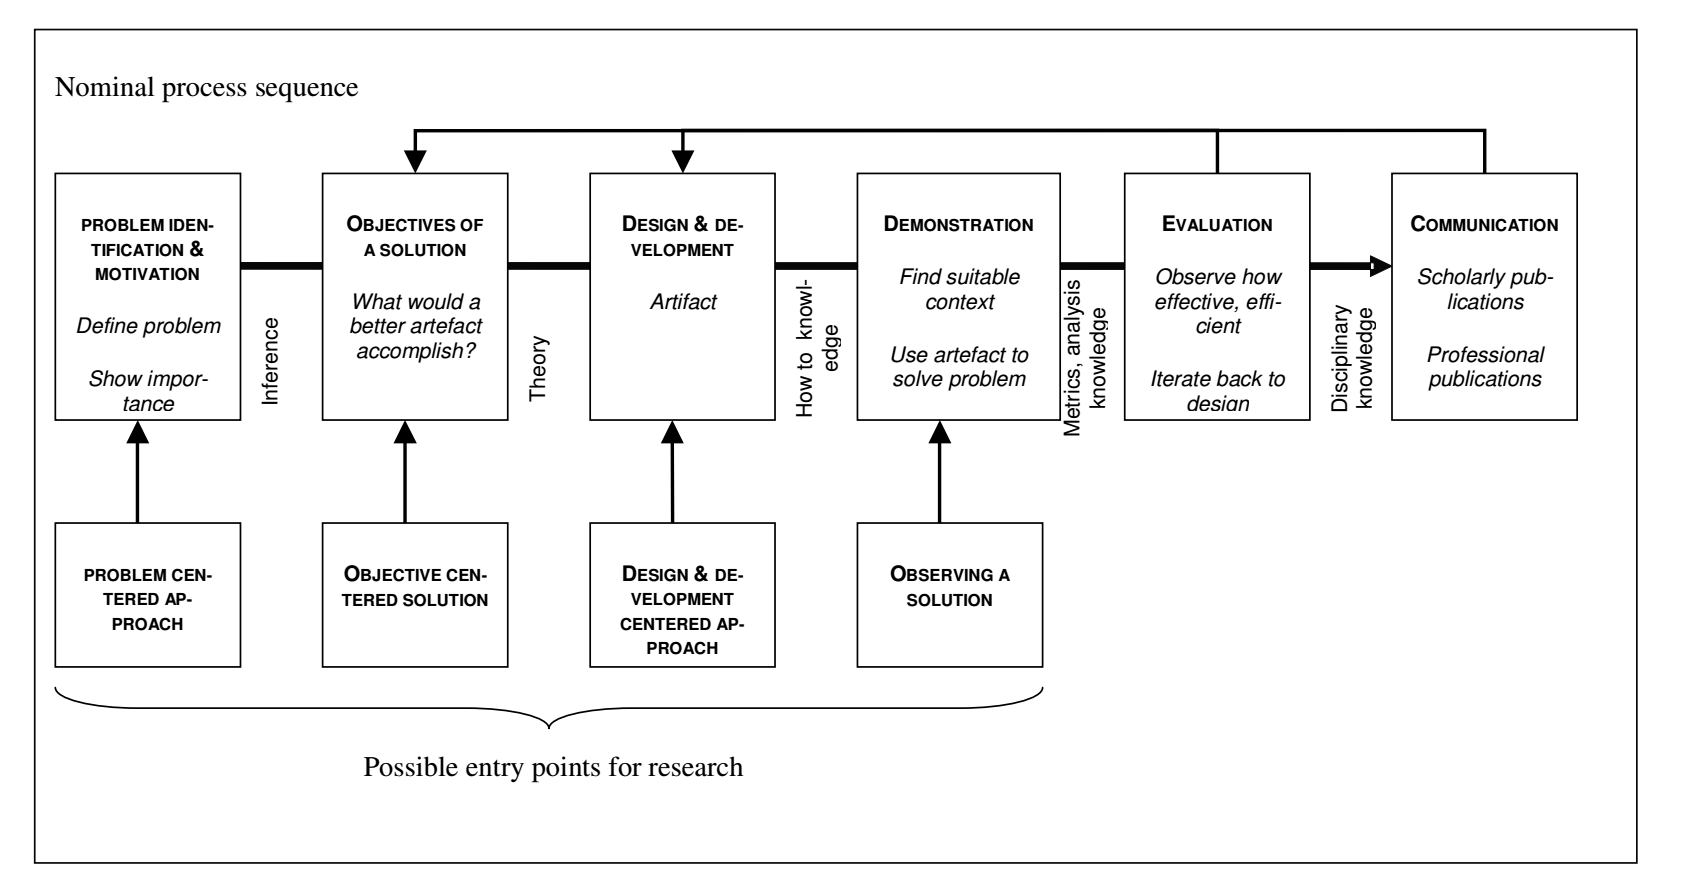
\includegraphics[width=\textwidth,center]{dsrp_modell.png}
	\caption[Design science research process (DSRP) model]{Design research process (DSRP)
	model\cite{peffers2006design}}
	\label{fig:DSRP}
\end{figure}


% section research_method (end)

\section{Project Research} % (fold)
\label{sec:project_research}
In this thesis, the problem was 
identified and motivated prior to the thesis, thus the natural starting 
point of this research was to go into the second stage; objective 
centered. \Ref{fig:DSRP} shows four entry points into a design 
research process; Problem centered-, objective centered-, design \& development-
centered-approach and observing a solution. \\

\textbf{Objectives of a solution} - This thesis was an interaction between objectives of a solution, and a study 
of prior art. Examining the state-of-the-art and existing systems is done by 
searching for scientific articles and commercial systems which contribute 
towards the goal of the thesis, and has been performed as a part of the 
background study. We are able to detect the holes in the available 
functionality, by describing and categorizing the systems found in the case 
study. As part of defining the objectives of the solution, we compared the 
provided functionality of the systems with the stakeholders and their 
requirements.\\

Two workshops were held as part of defining the goals of the solution and the 
prototype for step 2, define the needs of the stakeholders, and as part of the 
requirements elicitation. Several stakeholders were participating in these
workshops helped to define the direction of the process. By using a focus group 
consisting of stakeholders, we were able to define specifications for the 
system and the domain. 
%We are also guaranteed the if the specification is implemented as a machine which is subsequently connected to the environment, then the requirements will be satisfied \cite{zave1997four}. 


By putting together a focus group, one can utilize stakeholders to define the
objectives of a solution. As Nielsen \cite{FocusGroupstoStudyWorkPractice} 
describes, focus groups can be a great way to learn about the work that occurs 
"between" and "around" the solutions. Focus groups have the advantage of allowing more natural interactions between people than interviews.
By bringing together several users leads to spontaneous ad ideas \cite{nielsen1997use}. To ensure that these focus groups stays 
focused during the entire workshops, the moderator has to make sure the 
groups discusses a pre planned set of issues and set goals for the kind of 
information to be gathered. The use of focus groups within requirements 
engineering have become more popular, because of their claim to greatly 
accelerate the development of requirements \cite{goguen1993techniques}. \\

\textbf{Design and development} - A prototype were to be implemented, to help
answer the research question. In order to implement the prototype, a set of 
goals for the prototype was defined with the help of the case study and the 
workshops held in step two, presented in \Ref{sec:intro_research_question}. The
final design of the prototype is presented in \ref{cha:implementation}
\nameref{cha:implementation}.\\


\textbf{Demonstration \& Evaluation} - As part of the iterative process loop, pilots with the supervisors were performed each week. During these meetings the current status of both the case 
study and development of the prototype was demonstrated. The demonstrations 
were performed as the observational evaluation method case study, where the 
artifact is studied in depth in business environment \cite{von2004design}. The 
evaluation involves comparing the objectives of the solution to actual 
observed results from use of the artifact in the demonstration 
\cite{peffers2006design}, and was performed as a comparison of the prototype's 
functionality with the solution objectives defined in step 2. \\


% section workshops (end)

% chapter research_questions_and_method (end)


% !TEX root=../thesis.tex

\chapter{Background}
\label{chapter:background}

A train network is a complex system. Almost every running train have the 
possibility to affect almost every other train running in the system.  When 
you look at a busy area, such as a major city and it's closest
area, a great deal of trains can be on the move at any given time on a
railway network with limited capacity. This leads to limited time slots for each 
train and every problem can lead to major delays.


Even though one train may be experiencing delay, this delay may be part of a
sequence of problems that can be tracked back to a seemingly unrelated part of
the the network and a perhaps a bad decision there\cite{cule2011mining}. \\

In the Norwegian railroad a train is on schedule if it arrives the final
destination within a margin on 3 minutes and 59 seconds, if it is a long
distance train the margin is 5 minutes and 59 seconds. 
Jernbaneverket (see\vref{sub:subsection_jernbaneverket}) defines regularity as the number of trains that gets run as 
planed in the time schedule. 
Uptime in regards to punctuality is defined by Jernbaneverket from the hours of delay\footnote{Hours of delay due to infrastructure excluded traffic	management and external conditions} caused by infrastructure relative to sum of planed train hours\footnote{Planed train hours (passenger and freight trains)} per year.
\cite{jernbaneverketPunklighetsTall}
\begin{equation} Uptime =
		\frac
				{
					\text{Train hours - Hours of delay}
				}
				{
					\text{Train hours}
				}\times 100 
\end{equation}\\

As Landex\cite{landex2009gis} says, there exist few GIS-approaches concerning
visualization of railroad capacity. Both the visualizations shown by Landex and
in section \vref{sect:backgroundExamples} only seems to take into consideration if
the trains are delayed, and the amount of delay. 

However, to minimize the delays all over the railway network, it may be necessary
to not only see that certain routes are delayed but also why it is delayed. To
be able to understand this, you need to be able to mine data from the railway
network administrator and have a good visualization tool to present it. 

\pagebreak
\section{Examples}
\label{sect:backgroundExamples}

\subsection{Zugmonitor}
\label{sub:subsection_zugmonitor}

In the Zugmonitor (see \vref{fig:zugmonitor}) example each long-distance 
trains in the German railway network has been plotted as a arrow on a German 
map. To illustrate the punctuality of each train, a colored circle has been 
added to each arrow if the train is delayed with varying color depending on 
how big the delay is. It has also been implemented a time line functionality 
to see how the trains are on each step of the routes. This time line 
functionality has both a play forward function and manually drag along the 
time line.

\begin{figure}[!htbp]
	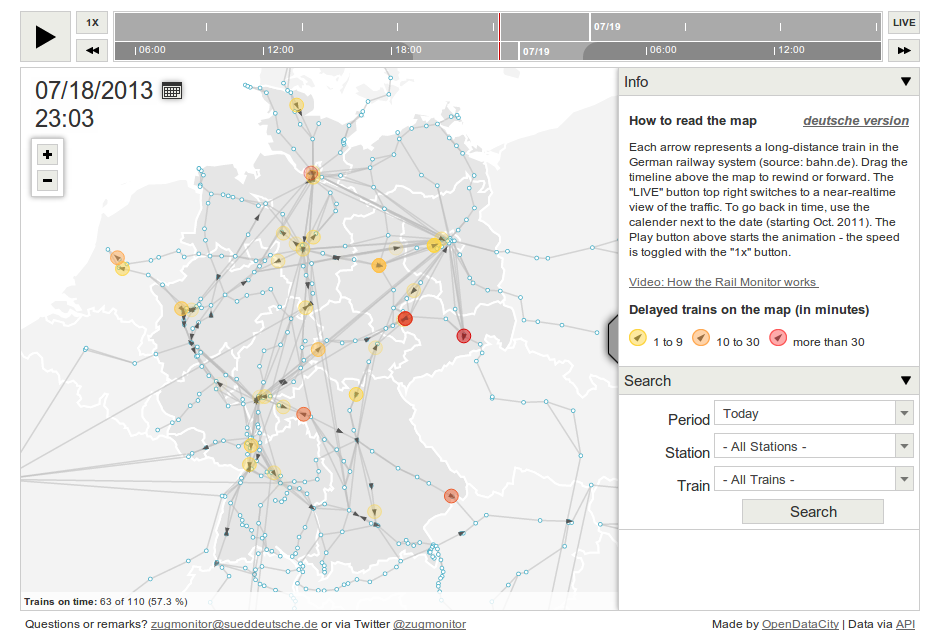
\includegraphics[width=\textwidth,center]{zugmonitor.png}
	\caption[Zugmonitor]{Zugmonitor \cite{zugmonitor}}
	\label{fig:zugmonitor}
\end{figure}
\pagebreak

\subsection{Vaguely live map of trains in the United Kingdom}
\label{sub:subsection_ukLiveMap}

This is a map which plots the relative location of each train in the United
Kingdom (see \vref{fig:ukLiveMap}). The plot fetches the departure time from the 
National Rail website and calculates the relative location. The plot does not
indicate whether or not the trains are on schedule or delayed, this must be
done either manually or for instance checking a time table\cite{trainTimesUK}.
Both the map and time table is developed on hobby basis by the same person. 

\begin{figure}[!htbp]
	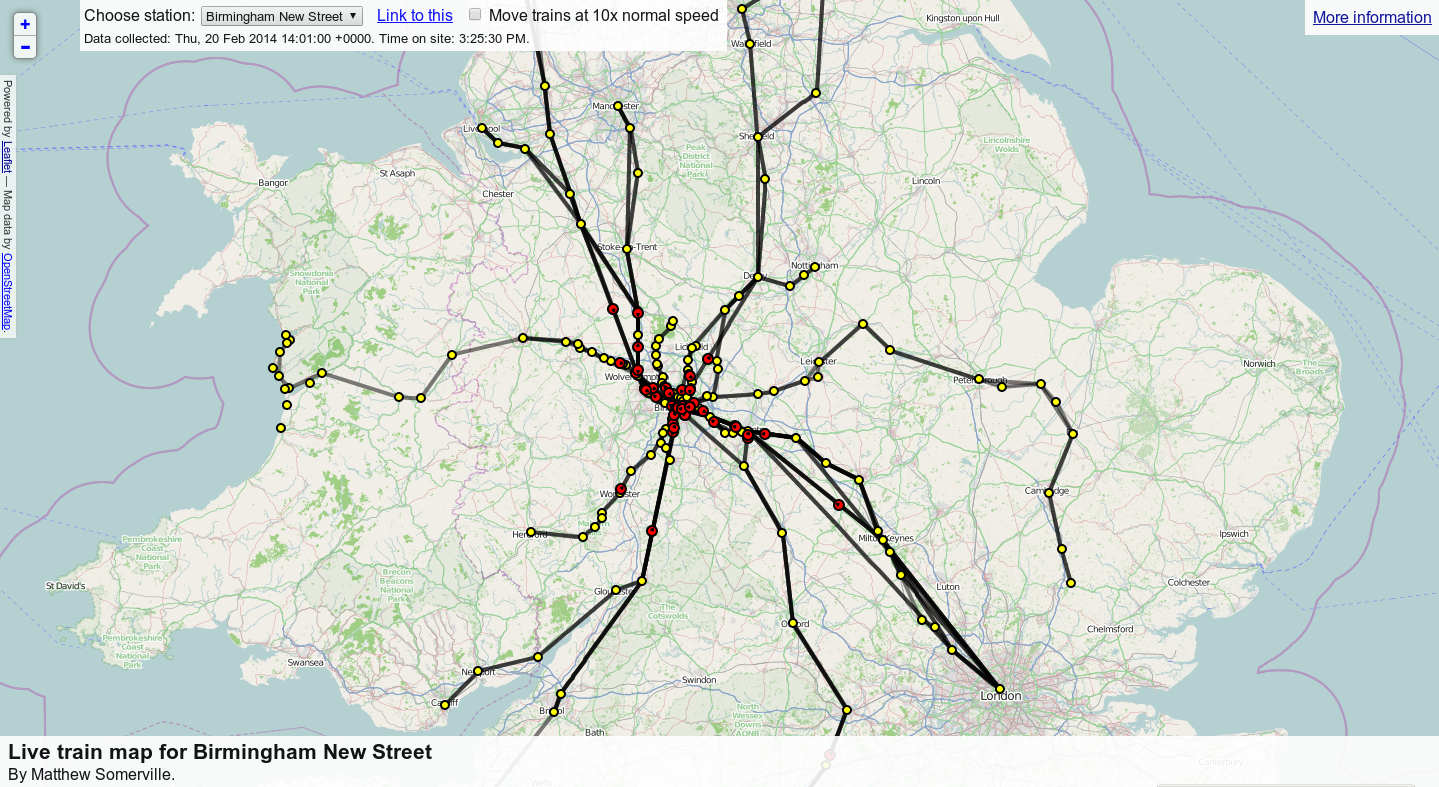
\includegraphics[width=\textwidth,center]{live-train-map-for-Birminingham-new-street.png}
	\caption[Vaguely live map of trains in the United Kingdom]{Vaguely live map of trains in the United Kingdom \cite{ukLiveMap}}
	\label{fig:ukLiveMap}
\end{figure}
\pagebreak

\subsection{MUNI Light Rail}
\label{sub:subsection_muniLightRail}

This a train graph based on the N-Judah line on the Muni Metro light railway line in San Francisco (see \vref{fig:muniLightRail}). 
This chart plots the schedule of the each train and the actual time each train 
uses. The chart auto updates each 10 seconds, and combined with being able 
to spot the difference between the schedule and the actual time, makes it easy 
spot the delay of each train. As with \vref{sub:subsection_ukLiveMap} it has been 
developed on a hobby basis.

\begin{figure}[!htbp]
	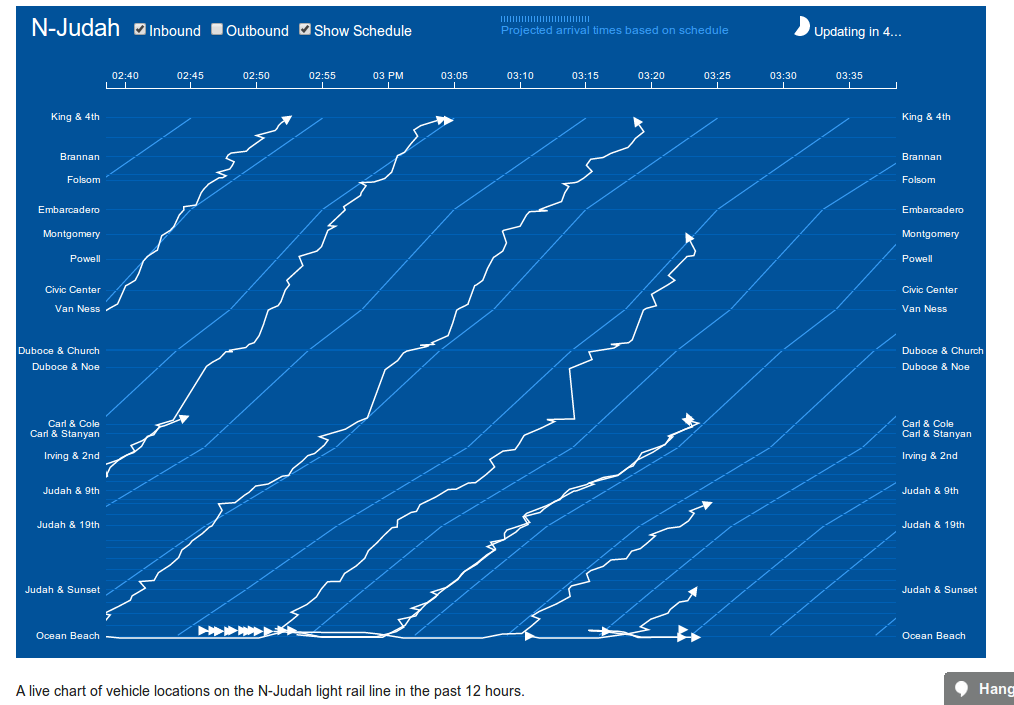
\includegraphics[width=\textwidth,center]{visualizing-transit-delays.png}
	\caption[Visualizing transit delays]{Visualizing transit delays \cite{muniLightRail}}
	\label{fig:muniLightRail}
\end{figure}
\pagebreak


\subsection{MiseryMap}
\label{sub:subsection_zugmonitor}

The MiseryMap (see \vref{fig:miserymap}) shows how much different airports and 
the routes between them are delayed. It also have a playback function to see
how the delays are throughout the day. This plot also shows some weather so it
may be possible to spot if the delays to be blamed on uncontrollable
conditions. 

\begin{figure}[!htbp]
	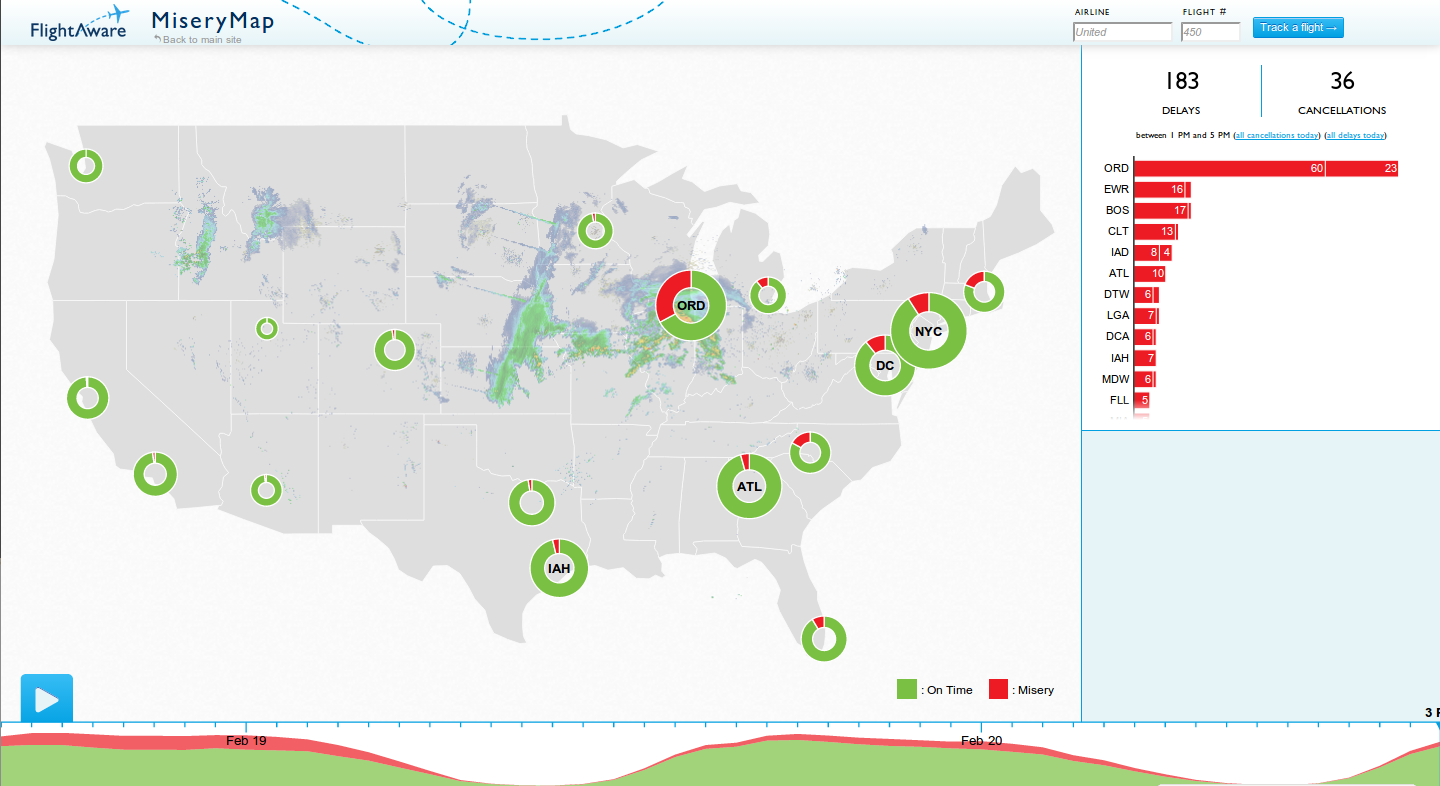
\includegraphics[width=\textwidth,center]{MiseryMap.png}
	\caption[MiseryMap]{MiseryMap \cite{flightAware:MiseryMap}}
	\label{fig:miserymap}
\end{figure}
%\pagebreak
 
\subsection{Jernbaneverket}
\label{sub:subsection_jernbaneverket}

Jernbaneverket is the Norwegian governments agency for railway services \cite{jernbaneverketAbout}.
This means that they are responsible for all the railway network in Norway.
Because of this, they also collect in data from points that each train passes. 
Based on this, they have recently released a map (see \vref{fig:jernbaneverket-punklighet}) over the punctuality on each stretch. This is a 
interactive map which shows a pop-up box containing the punctuality of the 
stretch clicked on, and this pop-up also shows which routes are using this 
stretch. The map, does not however, show more information if the user zooms 
inn, which is possible within the map itself, and has a static view of Norway 
and the railway. This map only shows the punctuality for passenger trains, and
not freight trains and/or both. 

To analyze each stretch, on a detail level of between each station,
Jernbaneverket has a internal system called TIOS (see \vref{fig:jernbaneverket-tios}).
This is a train graph which plots all trains that passes between all stations,
in this example between Oslo S and Drammen, where the red lines means delays
and the red circle indicates a reason code. XXX

\begin{figure}[!htbp]
	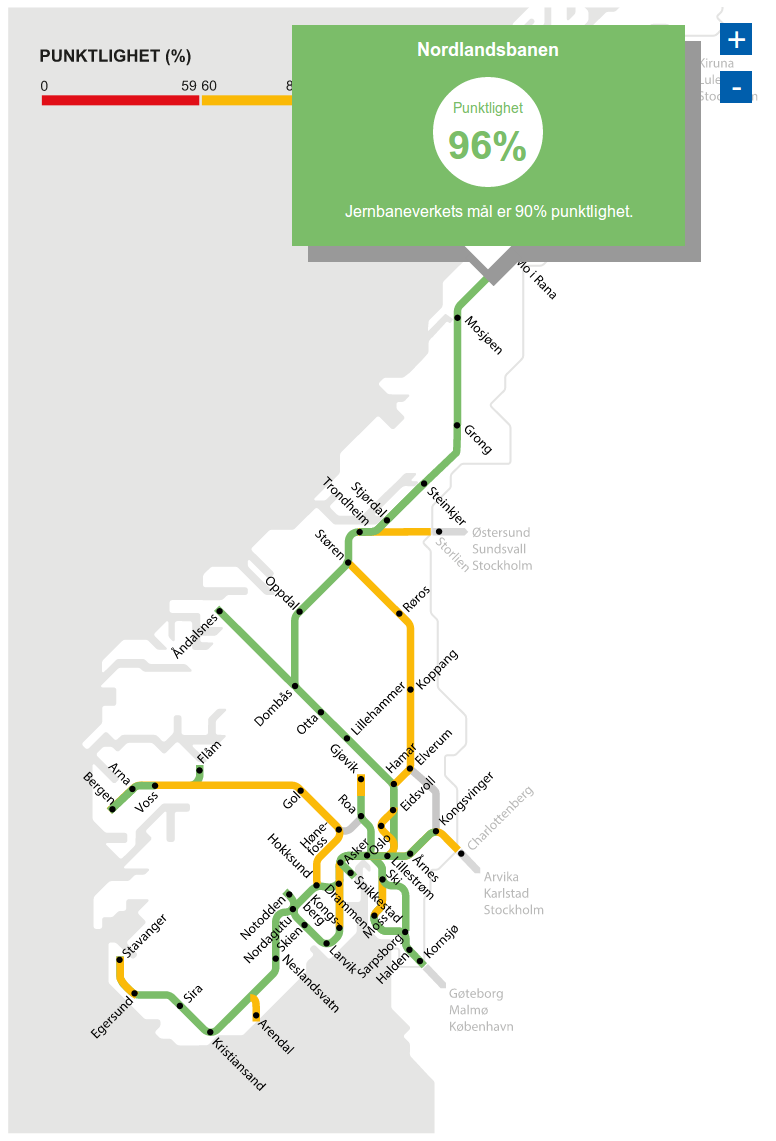
\includegraphics[height=\textheight,center]{jernbaneverket-punklighet.png}
	\caption[Punctuality map for Norwegian railway]{Punctuality map for Norwegian railway
	\cite{jernbaneverketPunklighetKart}}
	\label{fig:jernbaneverket-punklighet}
\end{figure}
\pagebreak

\begin{figure}[!htbp]
	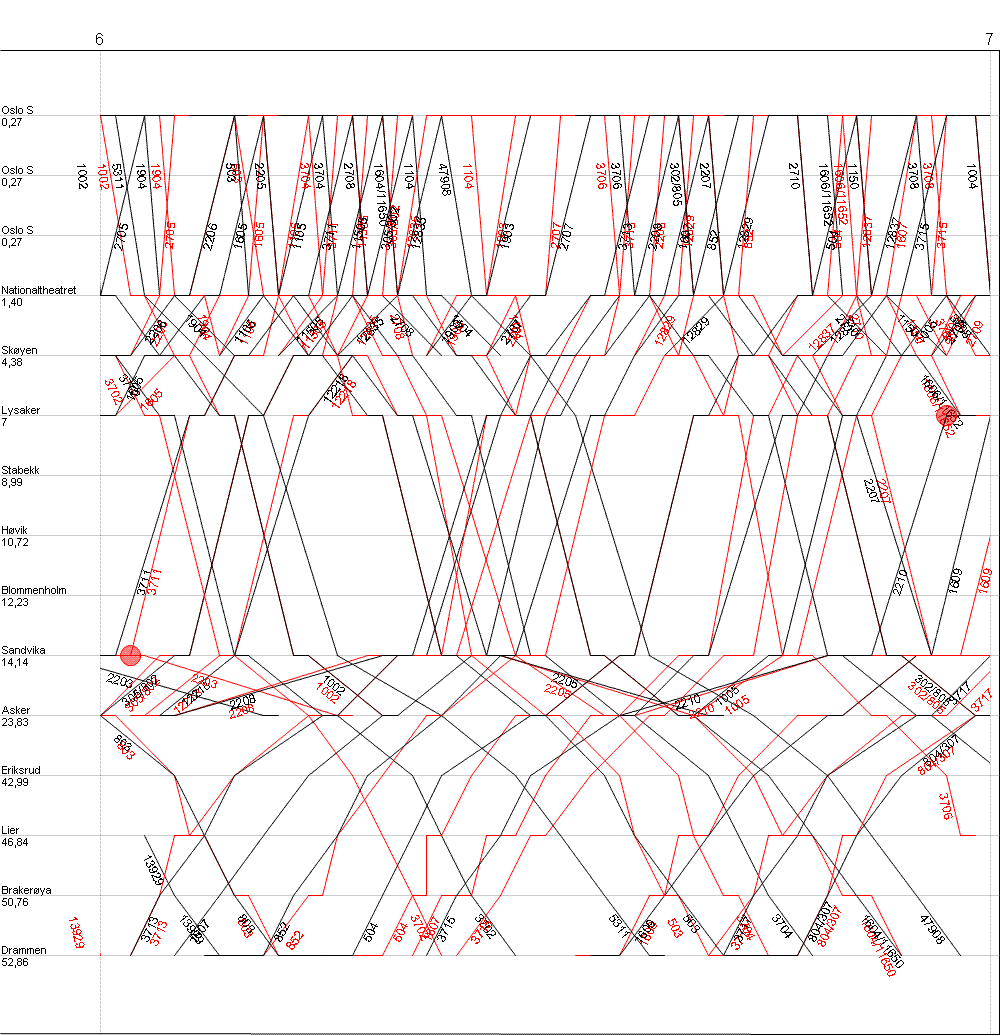
\includegraphics[width=\textwidth,center]{tios.png}
	\caption[TIOS]{TIOS\cite{jernbaneverketPunklighetKart}}
	\label{fig:jernbaneverket-tios}
\end{figure}
\pagebreak


\subsection{Tåg.info}
\label{sub:subsection_taag.info}

\begin{figure}[!htbp]
	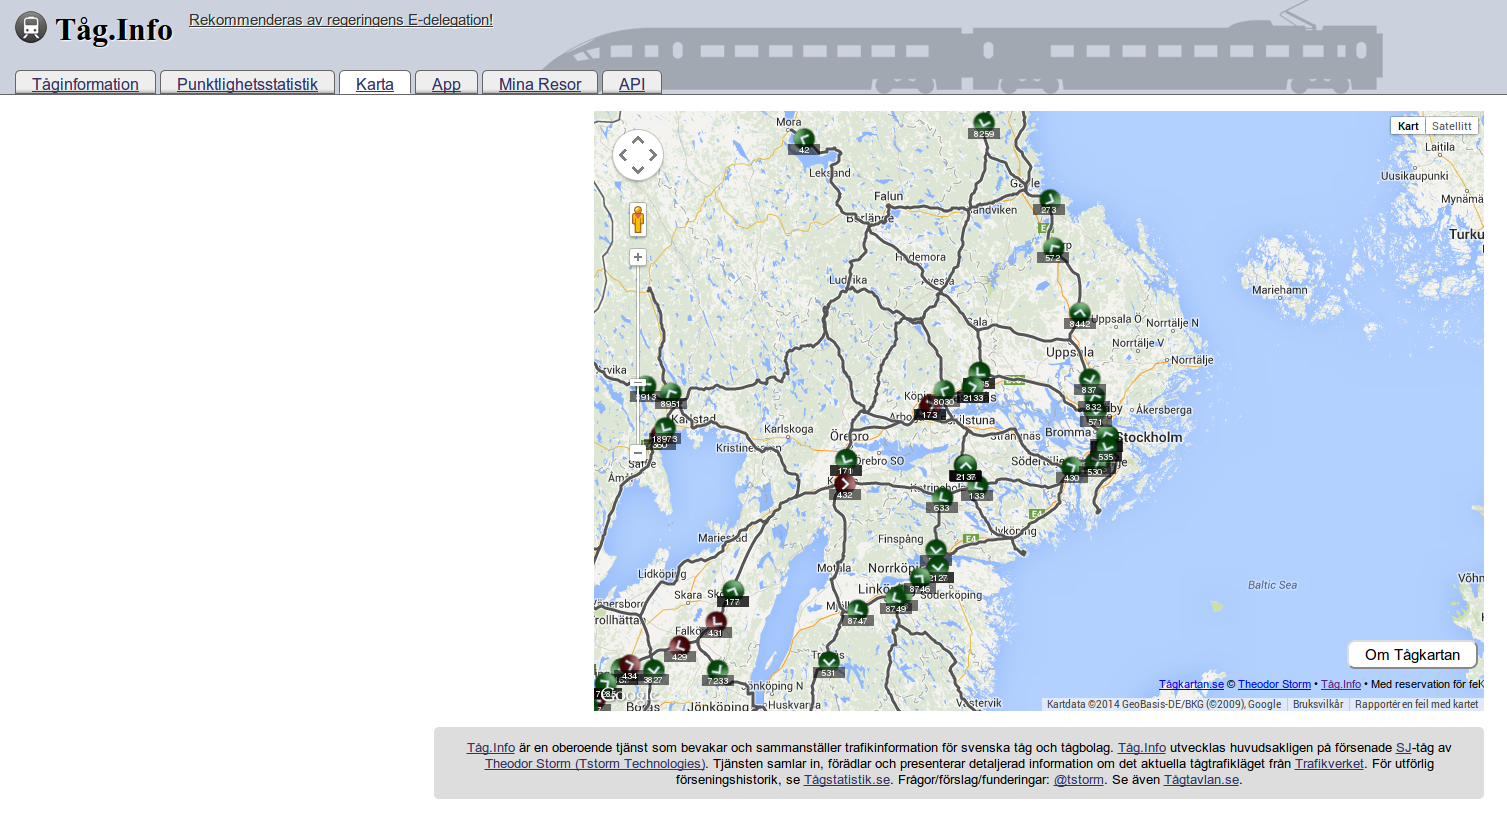
\includegraphics[width=\textwidth,center]{taag-info-kart.png}
	\caption[Tåg.info kart]{Tåg.info kart
	\cite{taagInfo}}
	\label{fig:taag-info-kart}
\end{figure}
\pagebreak

\begin{figure}[!htbp]
	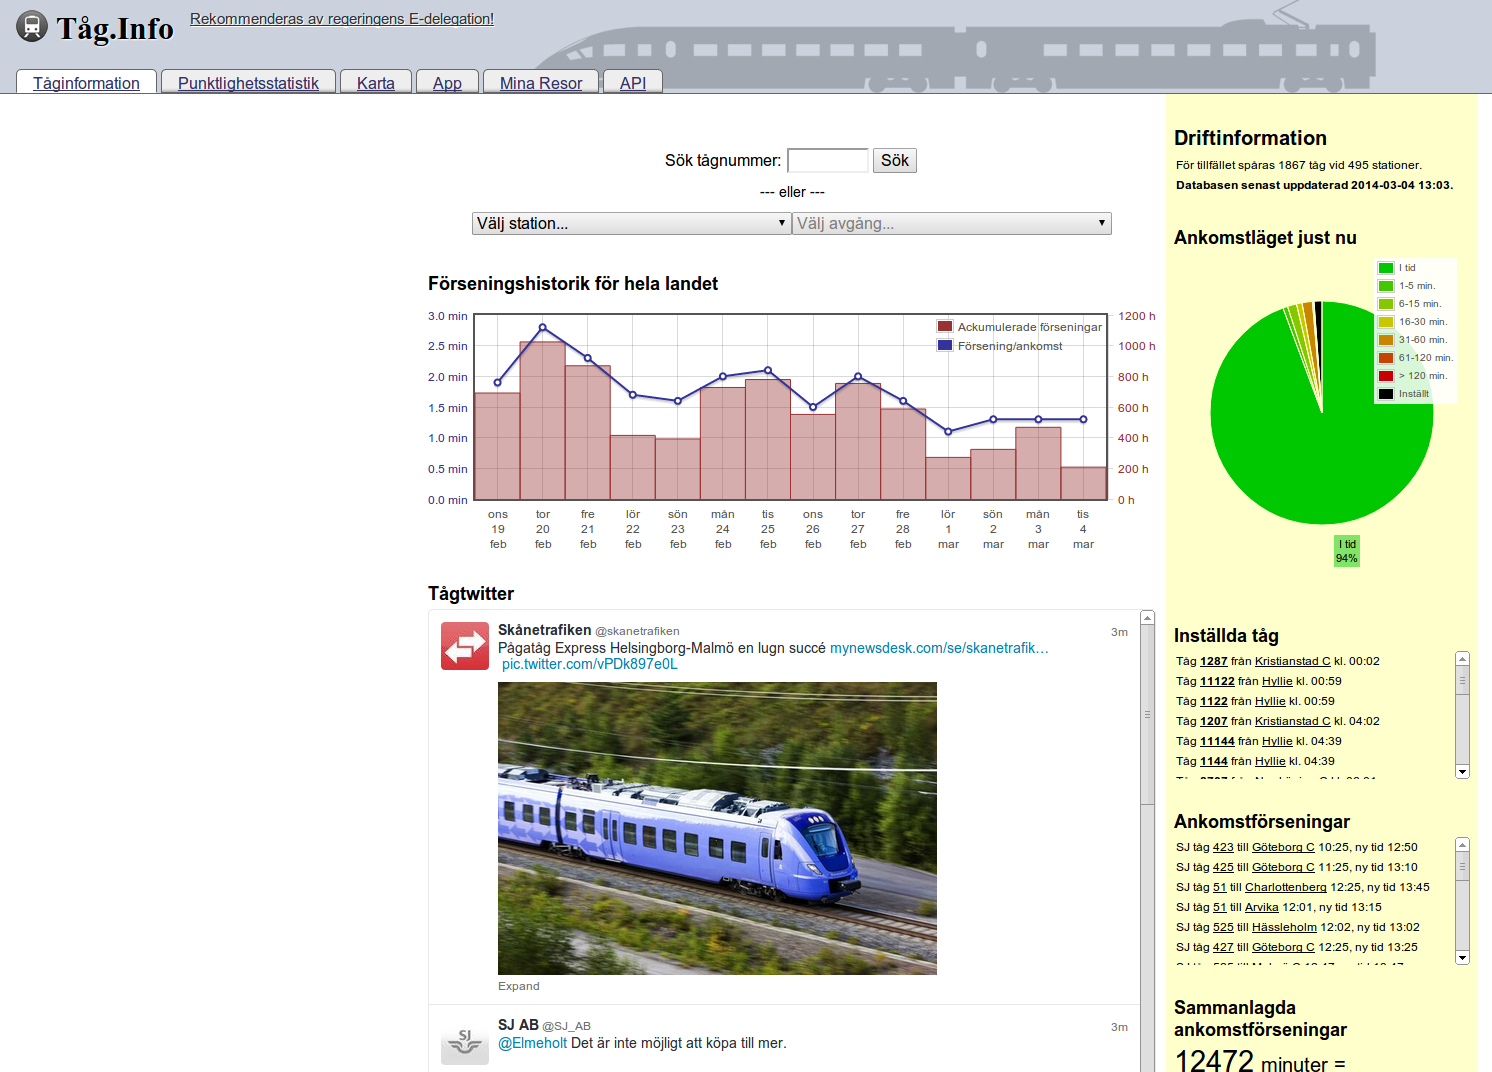
\includegraphics[width=\textwidth,center]{taag-info-historik.png}
	\caption[Tåg.info history]{Tåg.info history
	\cite{taagInfo}}
	\label{fig:taag-info-kart}
\end{figure}
\pagebreak


\subsection{SINTEF Presis}
\label{sub:subsection_sintefPresis}

The PRESIS\cite{sintefPresis} project is a project between SINTEF\cite{sintef},
Transportøkonomisk Institutt\cite{transportOkonomiskInstitutt},
NTNU\cite{ntnu}, Jernbaneverket(section \vref{sub:subsection_jernbaneverket}) and the train operators. It is meant to
systematicly improve the precision level in the railway system by developing
methods, tools, and processes. In this project it has been developed several
prototypes for analyzing train delays. 

If you look at \vref{fig:kjoretidstes-strekning}, it is possible to analyze the
difference in density between two selectable stations on two different,
selectable time periods. 

When looking at \vref{fig:krysningsinteraksjon}, it is possible to see how one
train might affect another at a selected station, plotted based on how much
both trains are delayed from -1 to 20 minutes. 



%\begin{figure}[!htbp]
%	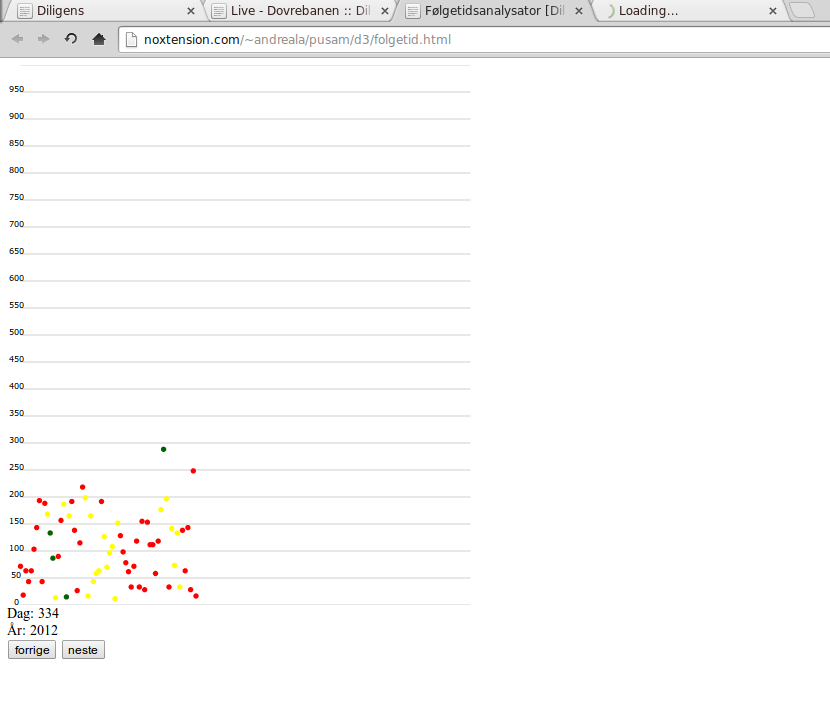
\includegraphics[width=\textwidth,center]{folgetid.png}
%	\caption[folgetid]{folgetid \cite{sintefPresis}}
%	\label{fig:folgetid}
%\end{figure}
%\pagebreak

\begin{figure}[!htbp]
	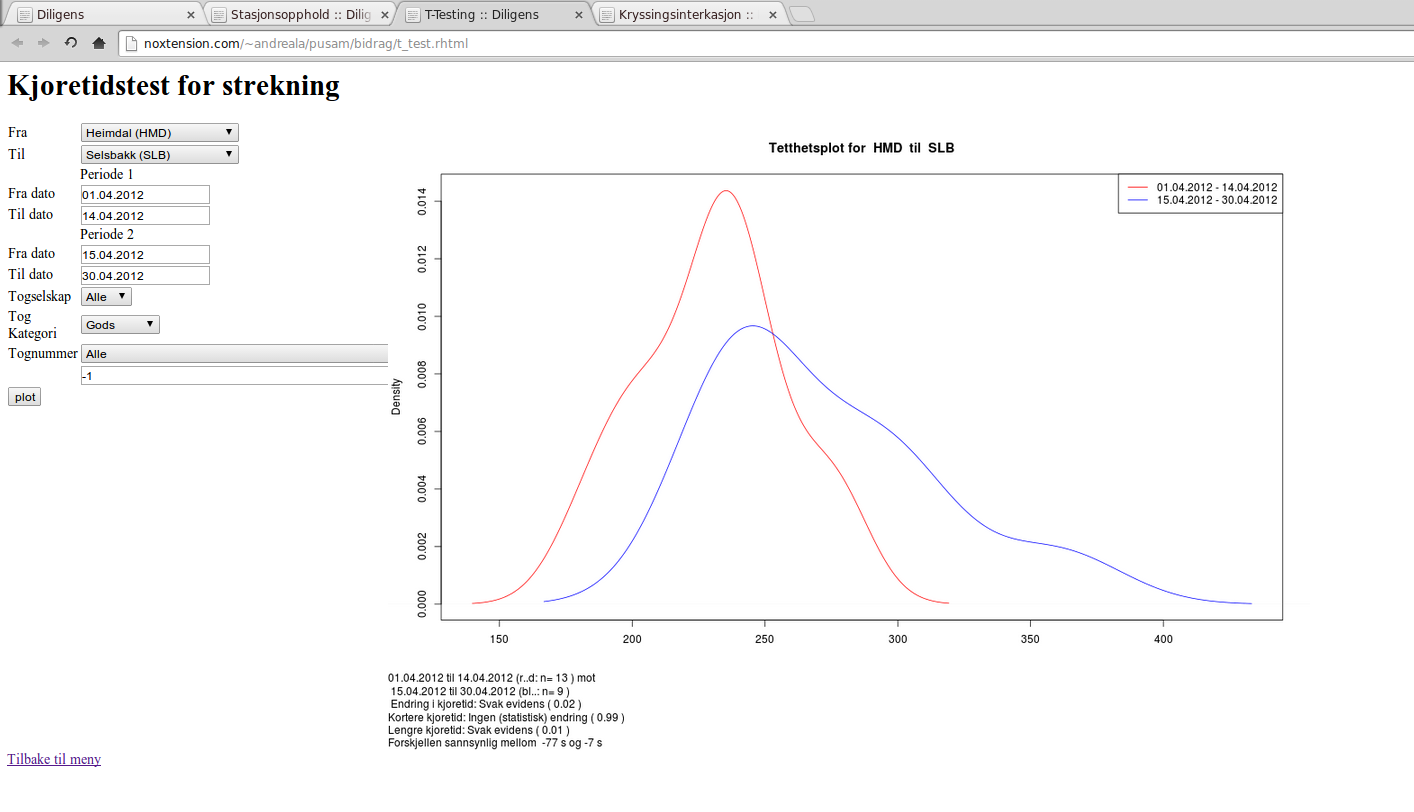
\includegraphics[width=\textwidth,center]{kjoretidstes-strekning.png}
	\caption[Density plot based on driving time]{Density plot based on driving time \cite{sintefPresis}}
	\label{fig:kjoretidstes-strekning}
\end{figure}
\pagebreak

\begin{figure}[!htbp]
	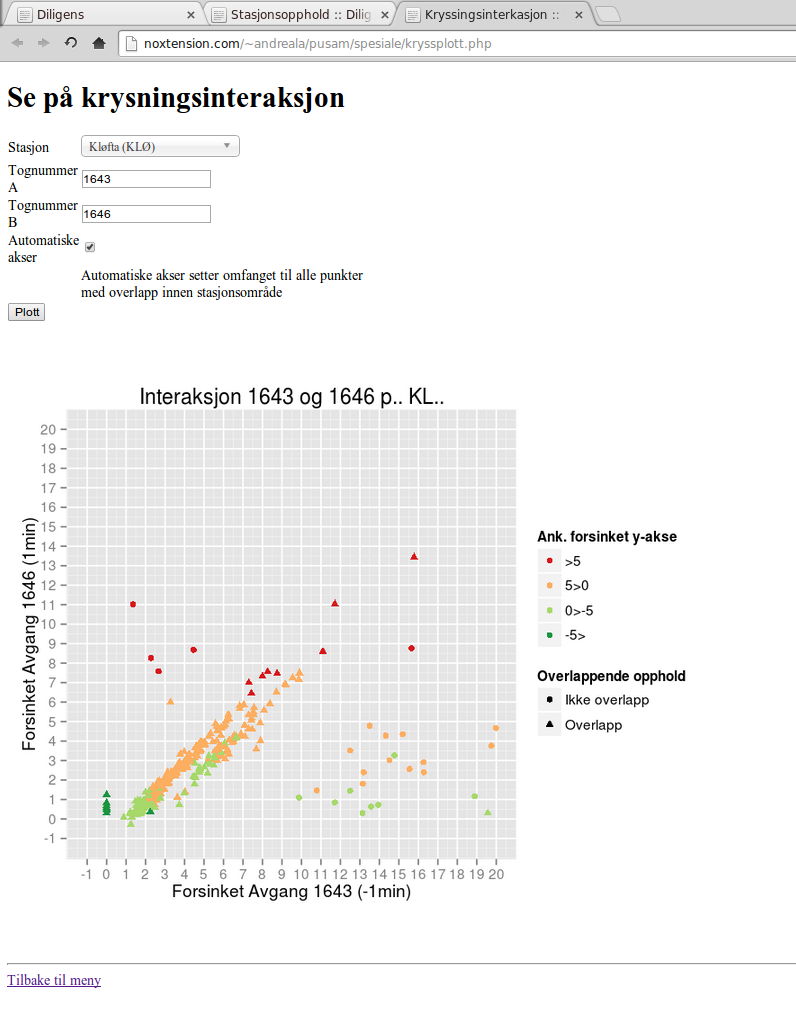
\includegraphics[width=\textwidth,center]{krysningsinteraksjon.png}
	\caption[Train interaction plot]{Train interaction plot \cite{sintefPresis}}
	\label{fig:krysningsinteraksjon}
\end{figure}
\pagebreak

\begin{figure}[!htbp]
	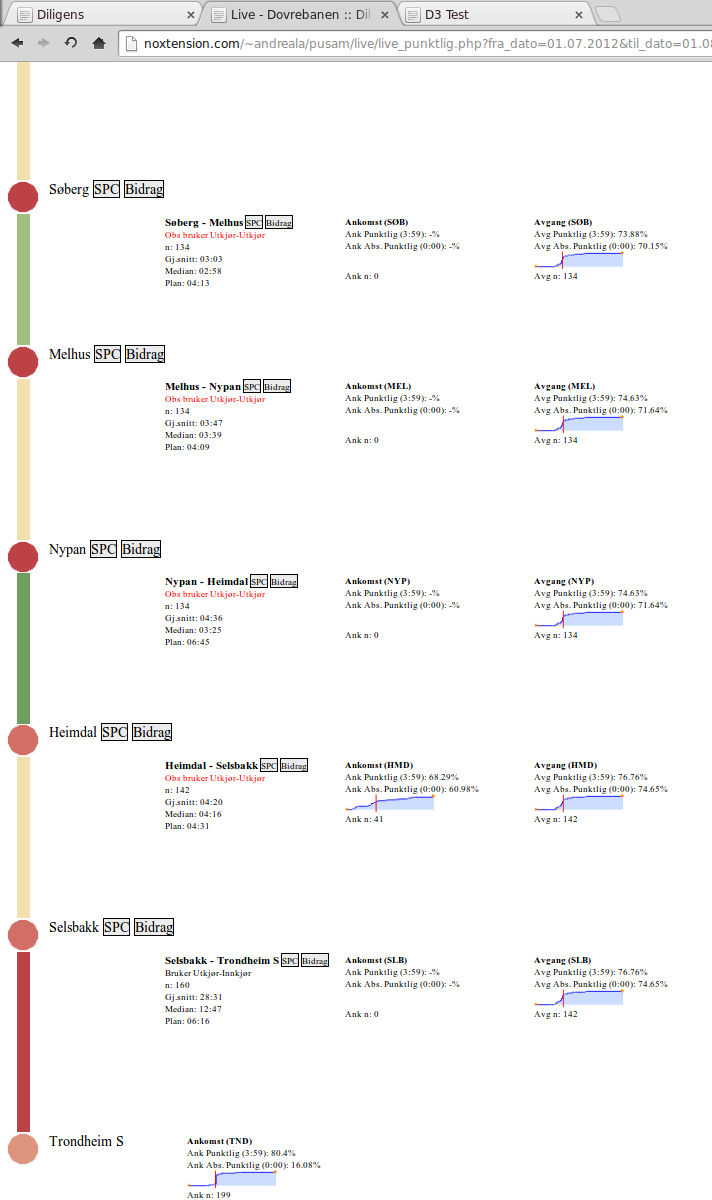
\includegraphics[height=\textheight,center]{live-punklighet.png}
	\caption[Punctuality for routes]{Punctuality for routes \cite{sintefPresis}}
	\label{fig:live-punklighet}
\end{figure}
\pagebreak

\begin{figure}[!htbp]
	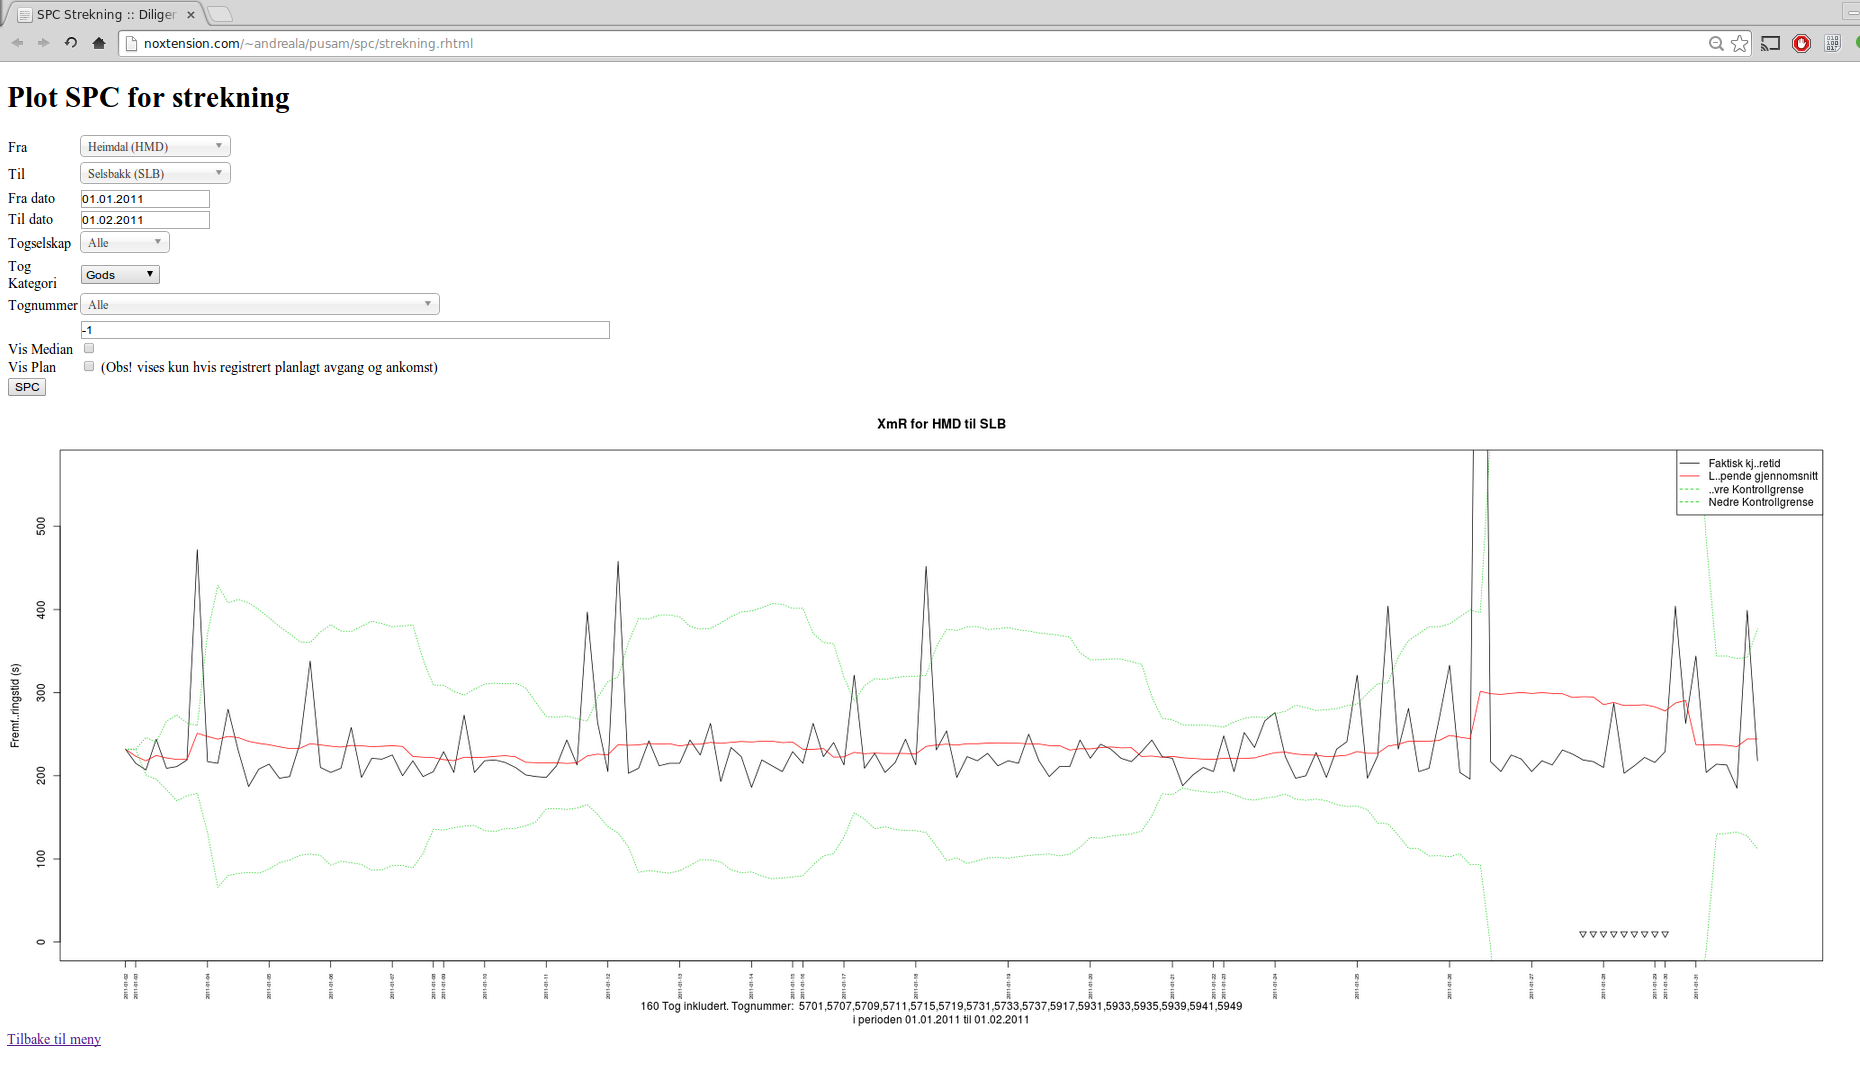
\includegraphics[width=\textwidth,center]{plot-spc-for-strekning.png}
	\caption[Time over distance plot (SPC)]{Time over distance plot (SPC) \cite{sintefPresis}}
	\label{fig:plot-spc-for-strekning}
\end{figure}
\pagebreak

\begin{figure}[!htbp]
	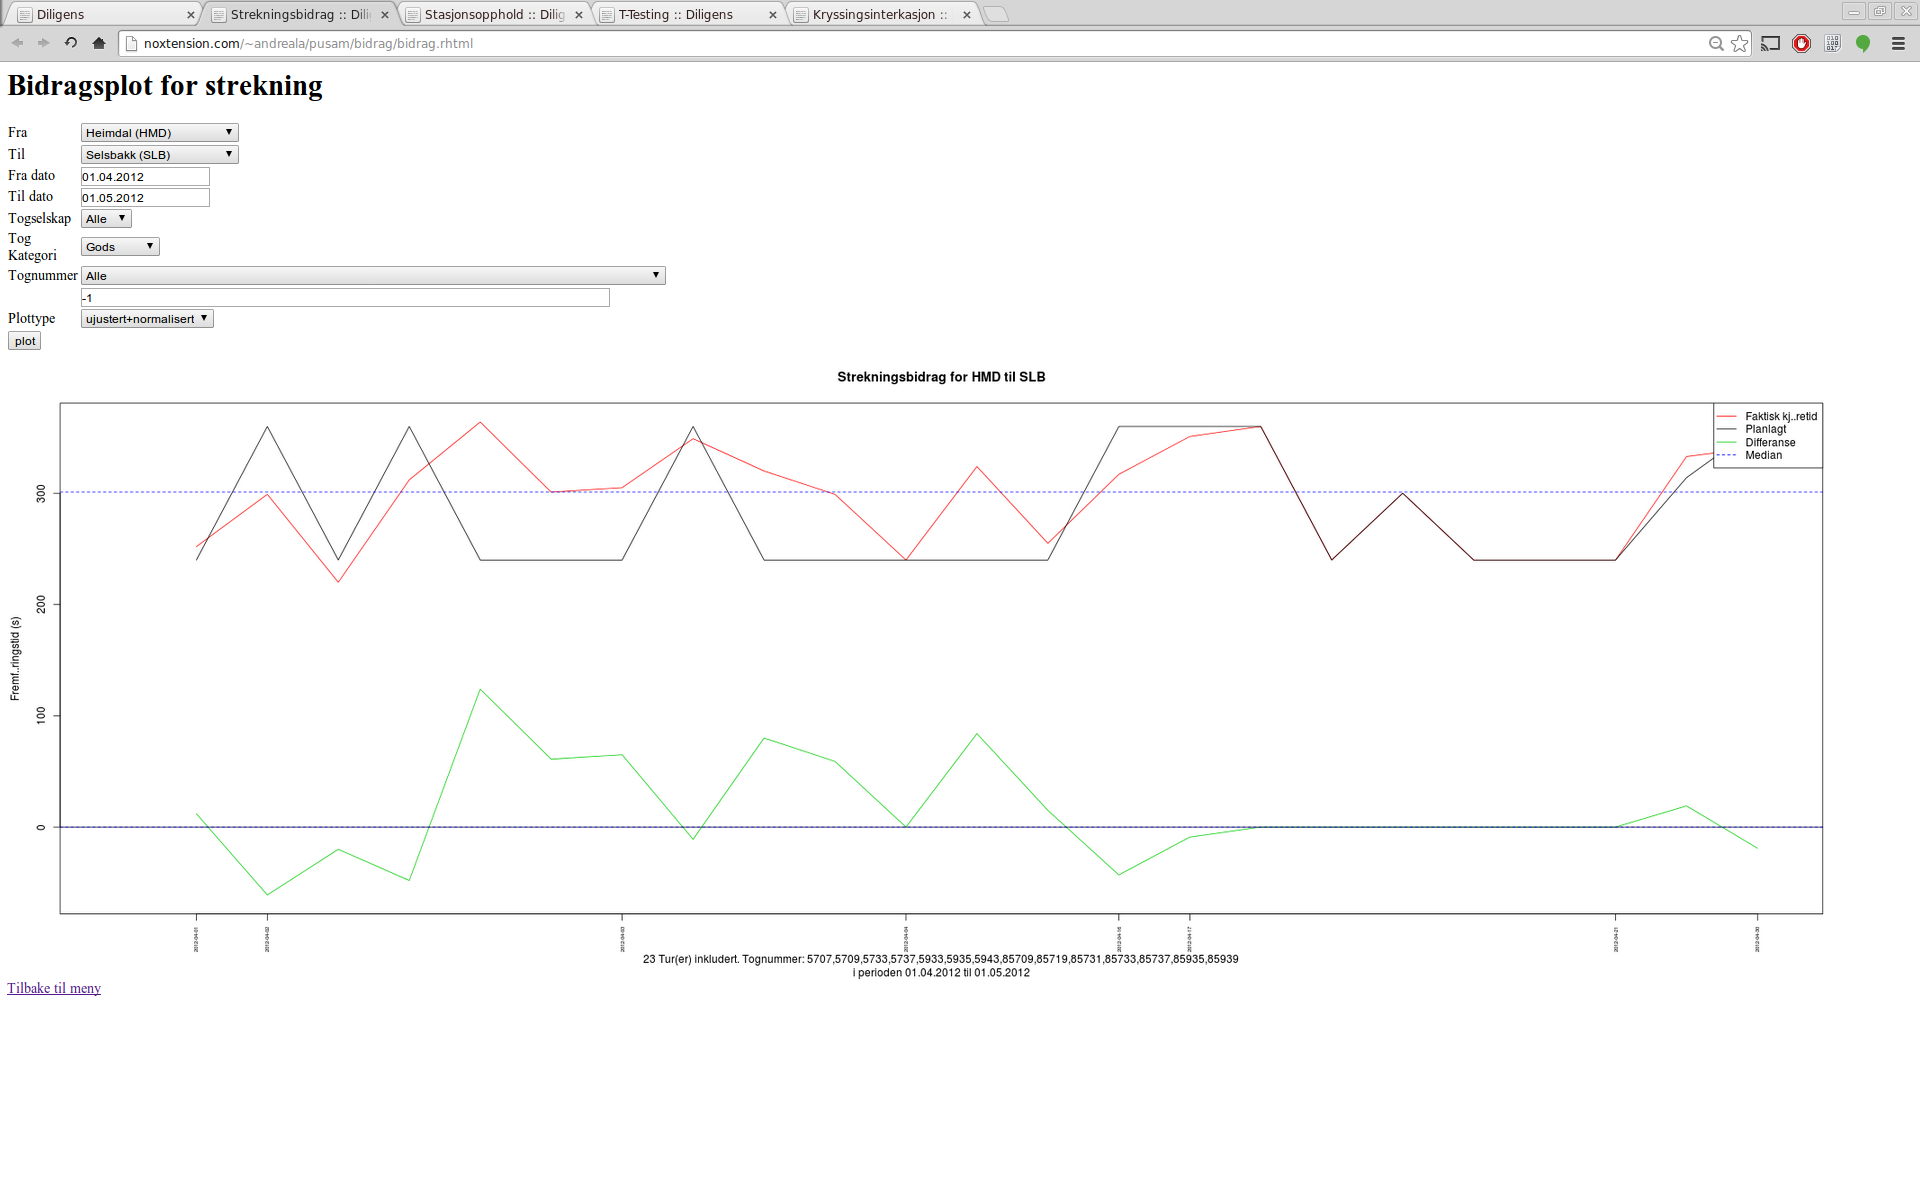
\includegraphics[width=\textwidth,center]{bidragsplot-strekning.png}
	\caption[Time over distance plot (Bidrag)]{Time over distance plot (Bidrag) \cite{sintefPresis}}
	\label{fig:bidragsplot-strekning}
\end{figure}
\pagebreak

\begin{figure}[!htbp]
	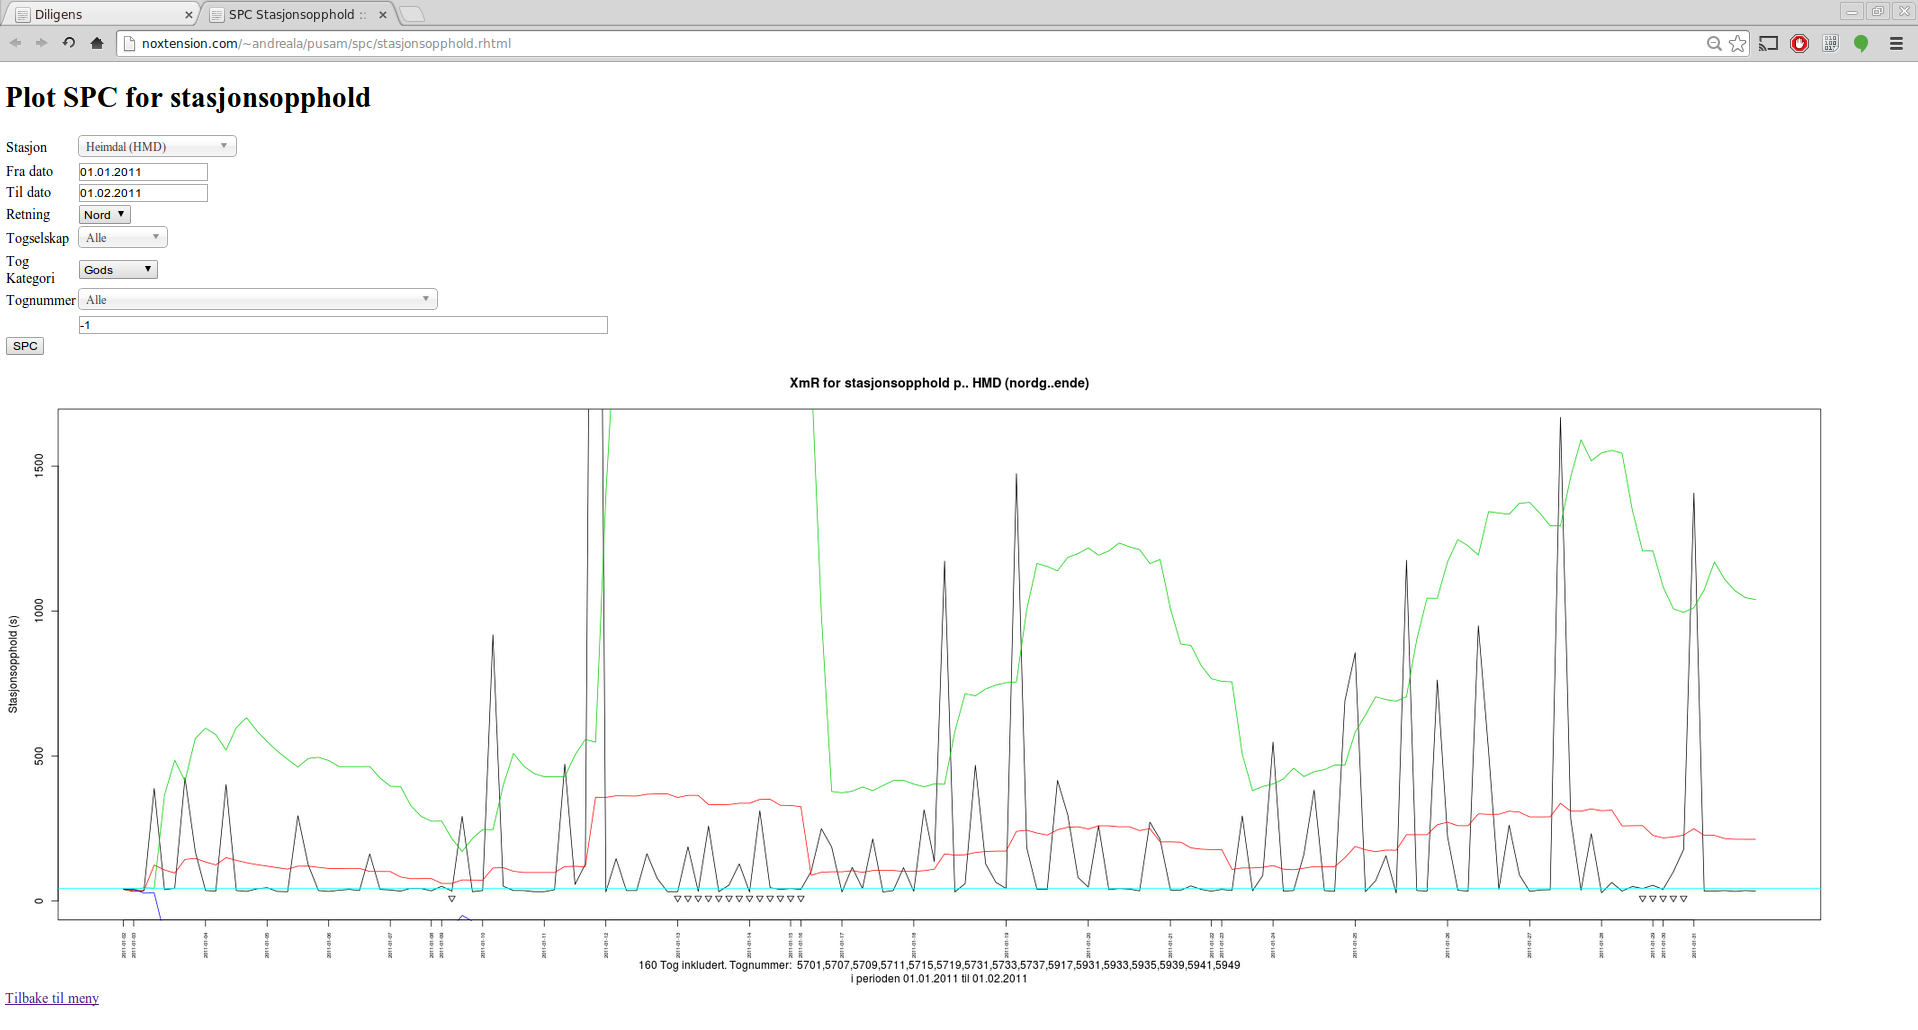
\includegraphics[width=\textwidth,center]{plot-spc-stasjonsopphold.png}
	\caption[Time at station (SPC)]{Time at station (SPC) \cite{sintefPresis}}
	\label{fig:plot-spc-for-stasjonsopphold}
\end{figure}
\pagebreak

\begin{figure}[!htbp]
	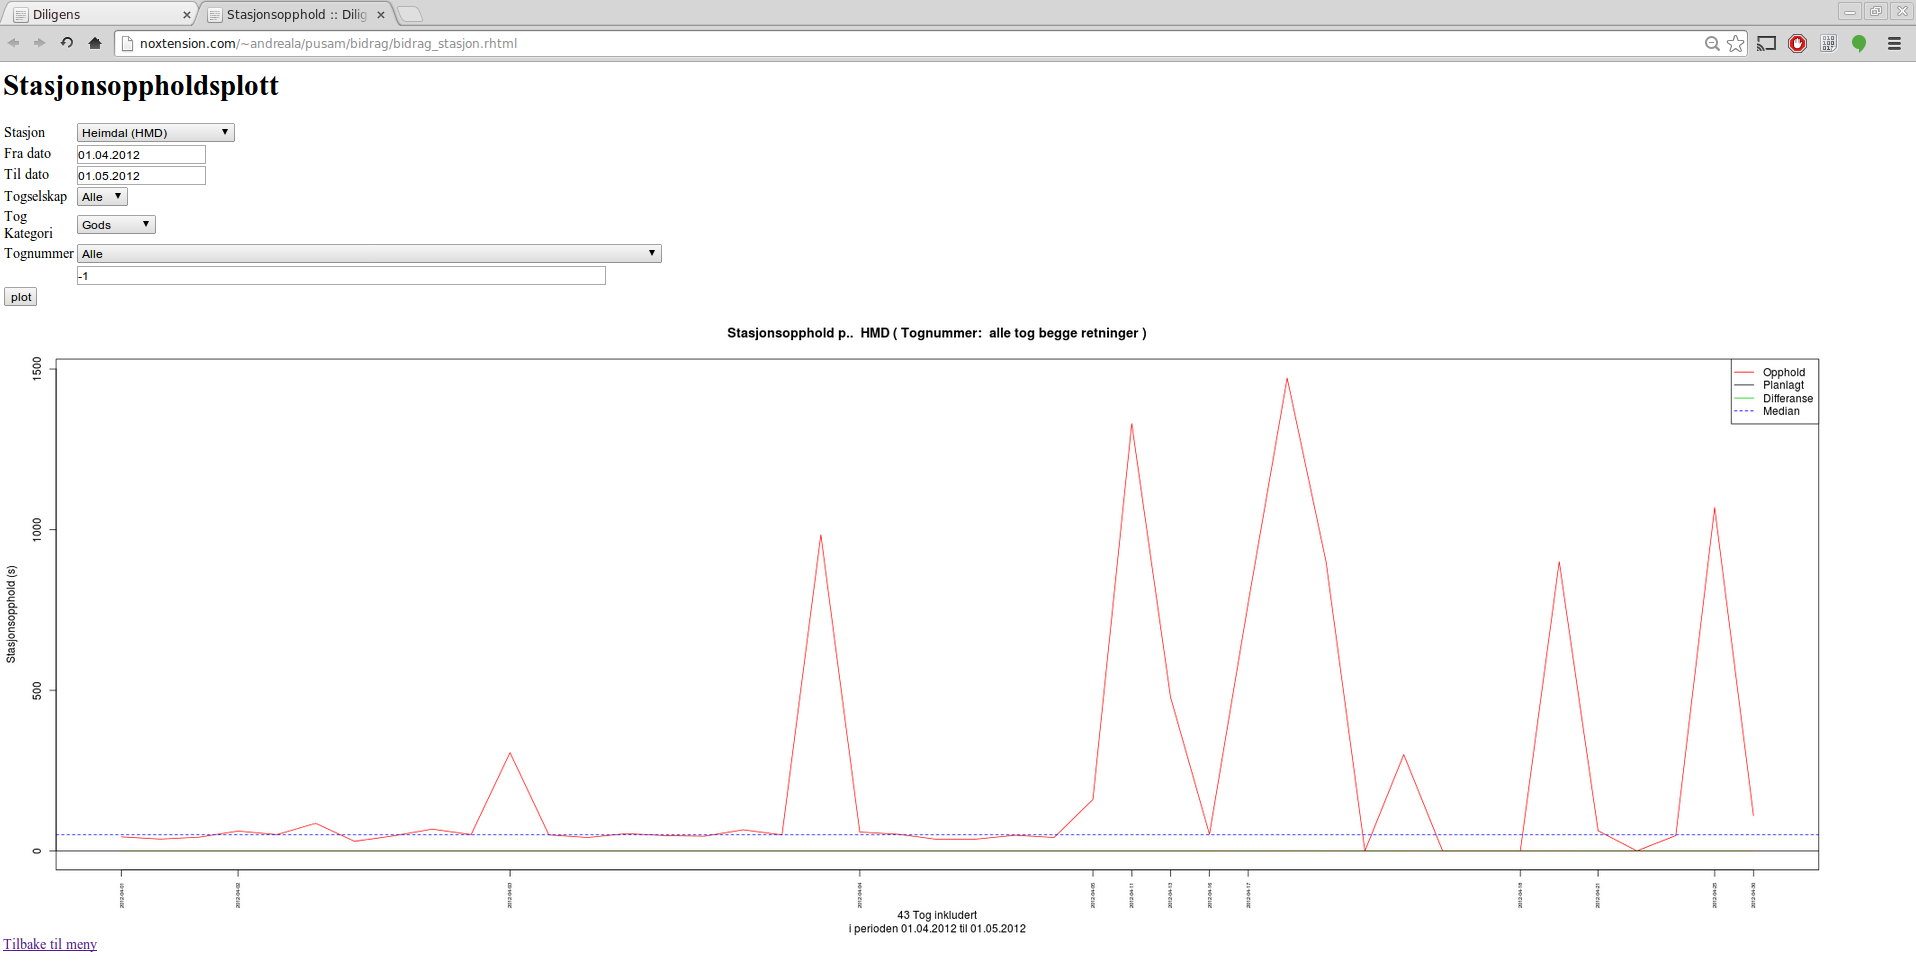
\includegraphics[width=\textwidth,center]{stasjonsoppholdplott.png}
	\caption[Time at station (Bidrag)]{Time at station (Bidrag) \cite{sintefPresis}}
	\label{fig:stasjonsoppholdplott}
\end{figure}
\pagebreak

\begin{figure}[!htbp]
	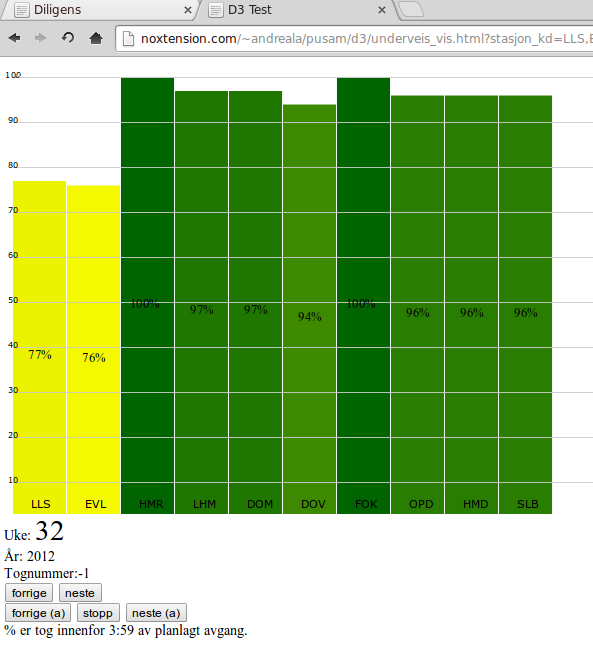
\includegraphics[width=\textwidth,center]{ukespunklighet.png}
	\caption[Weekly punctuality between stations]{Weekly punctuality between stations \cite{sintefPresis}}
	\label{fig:ukespunklighet}
\end{figure}
\pagebreak

\clearpage
\subsection{Cargonet} % (fold)
\label{sub:subsection_cargonet}

% subsection subsection_name (end)
Cargonet is a Norwegian which provides intermodal transport on rails. To 
provide a effective tracking service for the customers, Cargonet provides a 
internal service for the users which tracks all trains belonging to Cargonet.
As can be seen on \vref{fig:cargonet}, it only shows a picture of the current
status of each train, it lacks the possibility to analyze both each stretch 
individually  and analyze trains and stretches in time.

\begin{figure}[!htbp]
	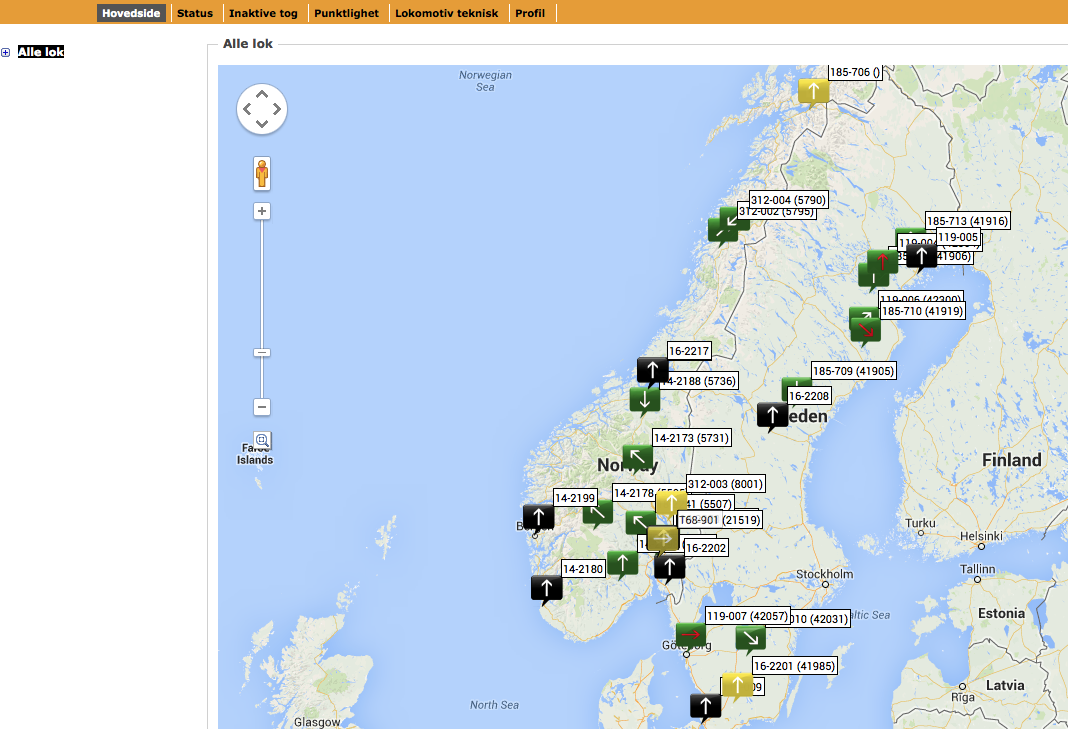
\includegraphics[width=\textwidth,center]{cargonet.png}
	\caption[Cargonet]{Cargonet \cite{cargonet}}
	\label{fig:cargonet}
\end{figure}

\begin{itemize}
	\item Red arrow:\hspace{4ex} Delayed.
	\item White arrow:\hspace{4ex} On time.
	\item Red box:\hspace{4ex} Locomotive driven 2km without carriages.
	\item Black box:\hspace{4ex} Locomotive without carriages.
	\item Yellow box:\hspace{4ex} Locomotive on time without schedule, or known position.
\end{itemize}

\pagebreak
% subsection subsection_cargonet (end)

%\chapter{Concept} % (fold)
\label{cha:concept}

% chapter concept (end)

% !TEX root=../thesis.tex

\chapter{Implementation} % (fold)
\label{cha:implementation}
In this chapter we will describe the technology used when developing the 
prototype, and how the technology was implemented. 

\section{Back-end} % (fold)
\label{sec:back_end}
In this section we will describe how the back-end of the system was 
implemented. The back-end is the part of the system which functions as the
interface between the user input from the front-end and data storages, and
mediates data between these.

\subsection{Data storage} % (fold)
\label{sub:back_end_data_storage}
Since the data was given in different sets and some sets serve a different
purposes, different sets was stored differently. For the prototype developed, 
the data was stored in 3 databases although optimally the amount of databases 
would have been two. The increased amount of databases is due to one of the data sets which was given as a interface to an existing database, while the others were given as sets which had to be put into a database.

The first database (The "station database") that was set up, was the one that 
contained the stations.
The structure was determined by the hierarchy of stakeholders presented in
\Ref{sec:back_stakeholders}.  We were presented with a list of all the
relevant stakeholders, which were all the area directors, stretch directors,
and segment director. The hierarchy in the "station database" database ended 
up as presented in the following list and the structure is similar for all 6 
areas and all the different numbers of stretches and segments beneath each 
area.

\begin{itemize}
	\item Area 1
	\begin{itemize}
		\item Strech 1
		\begin{itemize}
			\item Segment 1
		\end{itemize}
		\item Stretch 2
		\begin{itemize}
			\item Segment 2
			\item Segment 3
		\end{itemize}
	\end{itemize}
\end{itemize}


The second and third databases (the "information database(s)") were all built
around the stations. By having the databases built around the stations, the 
relation between these events and the stakeholders were a connection between 
the events and either one or two stations. Since all events had a connection 
to a station, these "information database(s)" all had a similar structure with 
data points such as stations where event occurred, scheduled and actual time 
of arrival and departure and train number. An example of such a data set is 
presented in \Ref{fig:jernbaneverket-trafikkdata}.

% subsection data_storage (end)

\subsection{Aggregation} % (fold)
\label{sub:back_end_aggregation}
When the system shall aggregate for the stakeholders, the front-end sends
the stakeholder, information type, and time parameters to the back end. 
The system then locates the correct stakeholder in the "station database",
which returns the correct area to which the stakeholder belongs. Based on the 
area returned by the database, the information selected, and the time window
selected, the system will fetch the relevant data from the "information 
databases". \\

Since most of the of the information is count based, the aggregation performed
on these sets are a simple average function along with generating dummy 
markers for each sub-area. Say one was to select a area as the current 
stakeholder with crossings as current data type, the system will then loop 
through and average all crossings per station within every segments and 
generate a marker located on the average location of all the stations with the 
average crossing of all these stations. The system will then do the same for 
all segments within one stretch. By performing the aggregation method for a 
area, you end up with a average marker for each stretch, located on the  
average location of all segments generated from all the stations, with the 
average crossings of all stations in that area.\\

The database structure presented above is implemented similar on the other 
sets of data, except in the case of Speed restrictions. The difference in the
datasets is due to that the workshops determined that the speed restrictions
was to be displayed with a own marker limited by the time selector.
% subsection back_aggregation (end)

% section back_end (end)

\section{Front-end} % (fold)
\label{sec:front_end}
In this section we will describe how the front-end was implemented. The
front-end is the part of the system that interacts with the user.

\subsection{Data set presentations} % (fold)
\label{sub:front_end_data_set_presentation}
When presenting the information to the user, the ability to maintain a tidy
presentation but at the same time present all the necessary information is 
important. Since the system shall present different kind of information, a 
selectable list of the implemented information types was implemented. The 
selectable list, presented in \Ref{fig:implementation_type_selection}, sets a 
internal variable which determines what kind of information shall be fetch 
from the databases and in turn be presented to the user.\\

As was mentioned in \Ref{sec:back_aggregation}, speed restrictions were
meant to be displayed as a own marker per event restricted within the selected
time window. In the database, each speed restriction event is stored with an id
which is equal to an image file with the plot. The data query will return with 
the id of each matched event, and the matching images will then be displayed
within the popup of the marker for each event. An example of a speed 
restriction marker with plot is presented in \Ref{fig:speed_restriction_presentation}.\\


Since the other information types were meant to be displayed in a dashboard, a
simple way of displaying the aggregated data along side each marker was made.
An example of a aggregated dashboard is presented in \Ref{fig:crossings_presentation} with the use of number of aggregated crossings in the Oslo area and East area as an example. When a user selects a new information type and the variable is updated, then sends a new request to the back end which in return presents the front-end with new data to present. The system will then dynamically update the dashboards and the markers.

When the time selection was to be implemented, the input method had been
decided to be implemented as input boxes in one of the corners for from and to 
date and time, as presented in\Ref{fig:time_selection_implemented}. When user 
changes the time interval, the input is validated to be in correct form and 
used in the request for data.\\

%TODO endre formulering på avsnittet her
It were also meant to implement a top 5 lists for each information, this was
however not completed. It was meant to display a list of the worst or best of
the information type within each current stakeholders responsible area. In the
case of crossings, the information would display the five stations with the 
most crossings, as demonstrated in \Ref{fig:top_5_list}. The top 5 list was 
demonstrated with static HTML-list of random stations with a random number.

When a request for information have been sent to the back end, the display will
then plot the information in markers. The system will then fit the map
according to a rectangle automatically calculated from the markers.
% subsection data_storage (end)

\subsection{Aggregation} % (fold)
\label{sub:front_end_aggregation}
Since most of the aggregation was done in the back end, there was not much
needed to be done in the front-end. One of the first things implemented, was 
the selection of stakeholders, see \Ref{fig:stakeholder_selection_list}. The
stakeholder is generated dynamically by sending a request for all the 
stakeholders to the back-end, and aggregate through the response which will 
generate the selectable list of stakeholders. 
% subsection back_aggregation (end)


\begin{figure}[h!tbp]
	\centering
	\begin{subfigure}{0.6\textwidth}
		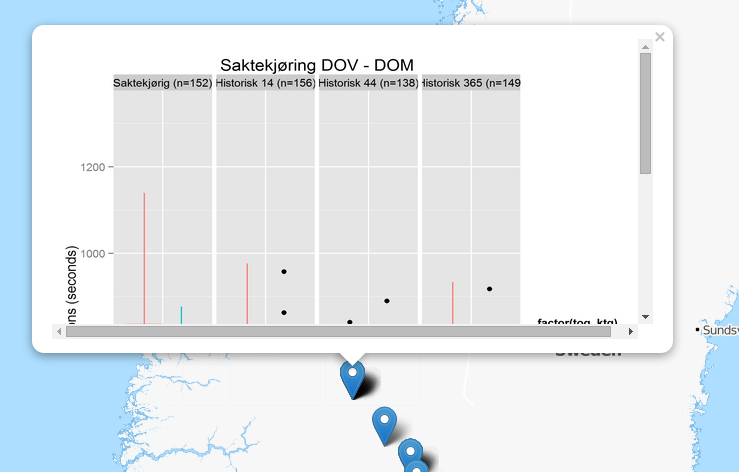
\includegraphics[width=\textwidth]{speed_restriction_presentation.png}
		\caption[Speed restriction presentation]{Speed restriction presentation}
		\label{fig:speed_restriction_presentation}
	\end{subfigure}
	\begin{subfigure}{0.25\textwidth}
		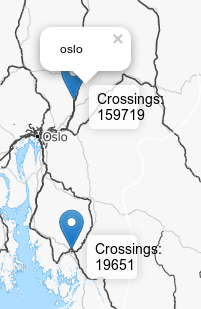
\includegraphics[width=\textwidth]{crossings_presentation.png}
		\caption[Crossings presentation]{Crossings presentation}
		\label{fig:crossings_presentation}
	\end{subfigure}
	\caption[Crossings and Speed restriction implementation]{Crossings and Speed restriction
	implementation}
	\label{fig:crossings_and_speed_restriction_implementation}
\end{figure}

\begin{figure}[h!tbp]
	\centering
	\begin{subfigure}{0.3\textwidth}
		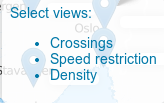
\includegraphics[width=\textwidth]{information_type_selection.png}
		\caption[Implementation type selection]{Implementation type selection}
		\label{fig:implementation_type_selection}
	\end{subfigure}
	\begin{subfigure}{0.6\textwidth}
		
\includegraphics[width=\textwidth]{time_selection_implemented.png}
		\caption[Time selection implementation]{Time selection implementation}
		\label{fig:time_selection_implemented}
	\end{subfigure}
	\caption[Information type and Time selection]{Information type and Time selection}
	\label{fig:information_type_and_time_selection}
\end{figure}

\begin{figure}[h!tbp]
	\centering
	\begin{subfigure}{0.4\textwidth}
		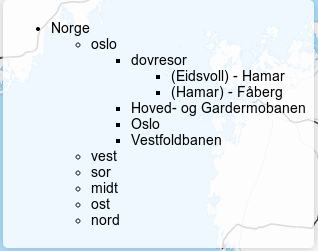
\includegraphics[width=\textwidth]{stakeholder_selection_list.png}
		\caption[Stakeholder selection list]{Stakeholder selection list}
		\label{fig:stakeholder_selection_list}
	\end{subfigure}
	\begin{subfigure}{0.4\textwidth}
		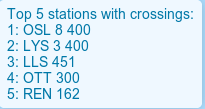
\includegraphics[width=\textwidth]{top5.png}
		\caption[Top 5 list]{Top 5 list}
		\label{fig:top_5_list}
	\end{subfigure}
	\caption[Stakeholder selection and Top 5 list]{Stakeholder selection and Top 5 list}
	\label{fig:stakeholder_selection_and_Top5_list}
\end{figure}

\begin{figure}[!htbp]
	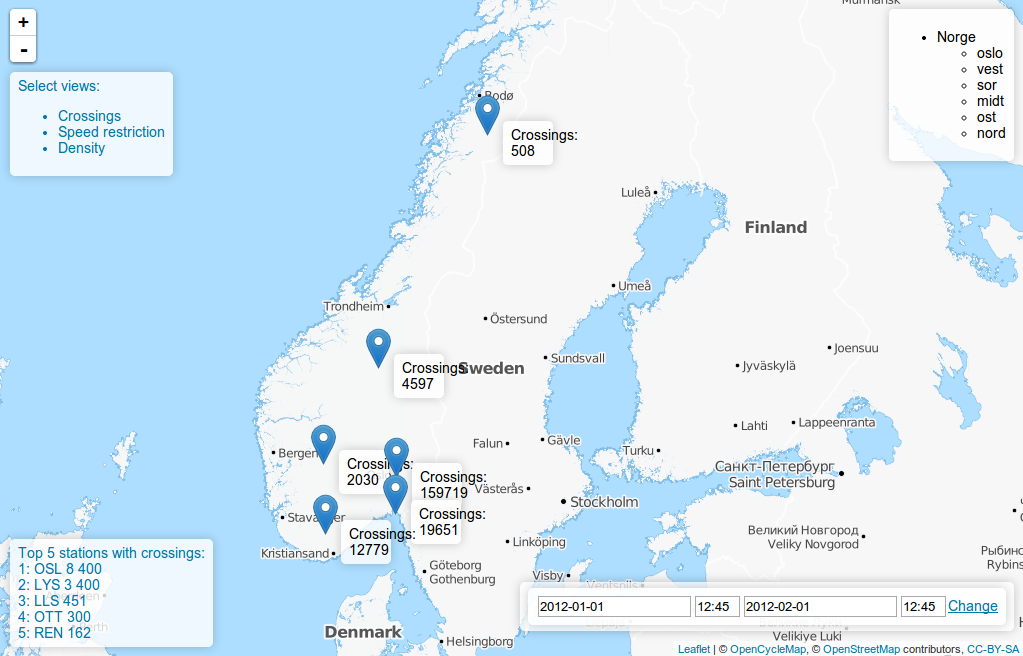
\includegraphics[width=\textwidth,center]{map_prototype.png}
	\caption[Map implementation]{Map implementation}
	\label{fig:map_prototype}
\end{figure}

% section front_end (end)

\section{Technology} % (fold)
This section will describe the technology used to implement the prototype.
\label{sec:technology}

\subsection{Server} % (fold)
\label{sub:server}
When the back end was due for implementation, Node.js\cite{nodeJs} was chosen 
as the framework for the server. Node.js is a event-driven, non-blocking  I/O
model framework which is based on Chrome's\cite{chromeJavaScriptEngine} 
JavaScript runtime. The Node.js framework enables small, fast, and scalable 
network applications.

When the user wanted to change information type or active stakeholder, the
request for data was posted to the server through a REST\cite{REST} api. An
example of a request for the number of crossings for the Oslo area is
"/rail/numberOfCrossings/2012-01-01/2012-02-01/oslo". The server then uses the
Express\cite{express} framework to parse all get request to the server to send
these request to methods within the Node server which parses these requests.


 % subsection server (end)

\subsection{Data storage} % (fold)
\label{sub:technology_data_storage}
When storing the data, several types of databases was used as mentioned in
\Ref{sub:back_data_storage}. The "station database" was implemented in
a noSQL document database structure called MongoDB\cite{mongoDB}. The MongoDB
database have a structure which on a database holds a set off collections. a
collection holds a set of documents. A documents is a set of key-value pairs.
For this thesis, The MongoDB database structure meant that one can search 
on a single key, for instance the name of an area, and get all relevant data 
within that structure. The MongoDB driver called Monk\cite{npmMonk} was used 
to access the implemented MongoDB database.\\

When setting up the last two databases, more traditional relational databases 
was used. The first database implemented was one in PostgreSQL
\cite{postgreSQLAbout}. The node-postgres\cite{node-postgres} was used to 
access this database. The PostgreSQL database was chosen due the functionality 
of the database and since we were most familiar with PostgreSQL. The 
last database was given as an interface to connect to, and was set up in MySQL
\cite{mySQLAbout}. The node-mysql\cite{node-mysql} driver was used to access 
the given MySQL interface.
% subsection technology_data_storage (end)

\subsection{Map} % (fold)
\label{sub:map}
Since the map was a important part of the presentation of data, the selection
of the map library were an important decision. Leaflet\cite{leaflet} was 
chosen due to the library being a more and more popular library which is open 
source. The Leaflet JavaScript library is designed with simplicity, 
performance and usability in mind.

All functions within the map is an extension of functions that exists in the
map. Information selection, time selection, stakeholder selection and Top 5 is
an extension of the L.Control object. The dashboards uses a standard marker,
and a bit of css to display the marker icon and the information. The map
prototype developed was presented in \Ref{fig:map_prototype}.
% subsection map (end)

% section technology (end)

% chapter implementation (end)

% !TEX root=../thesis.tex

\chapter{Results}
\label{chapter:results}
This chapter will present results found by performing activities described in
\Ref{cha:research_questions_and_method} \nameref{cha:research_questions_and_method}. 

In the two first parts we describe the results of the workshops held. The last 
part describes the functionality in the prototype developed. The implementation
of the prototype was described in \Ref{cha:implementation} \nameref{cha:implementation}.

% !TEX root=../../thesis.tex

\section{Workshop 2014-04-04} % (fold)
\label{sec:workshop_2014_04_04}
The first workshops agenda was to help define the stakeholders of the system,
their areas of responsibility, and their needs. The workshop was also meant to 
bring clarity to how the system will relate to these users and their needs.
Attending this workshop was Andreas Amdal Seim (SINTEF), Andreas Dypvik 
Landmark (SINTEF), Rimmert van der Kooij (SINTEF), Nils Olsson (NTNU), Per 
Magnus Hegglund (Jernbaneverket), Magnus Bae (NTNU), and Magnus Krane (NTNU).\\

Perspectives that can be used when viewing the system were discussed
first.
\begin{itemize}
	\item Infrastructur: Segment director, etc.
	\item Traffic division / passenger / train companies.
	\item Delay causes: delay demographic.
\end{itemize}

Interests of users when using the system were then discussed based on the
perspectives.
\begin{itemize}
	\item Uptime, punctuality.
	\item Deviation.
	\begin{itemize}
		\item What?
		\item Where?
		\item When?
	\end{itemize}
	\item Delay time.
	\item Variation.
	\item Changes.
\end{itemize}

Causes that might affect the punctuality was also listed: weather, number of
passengers, capacity utilization, animal accidents, cargo volume.
The causes was concluded not to be included in this project, as the causes is
difficult to prove and get data on.\\

The internal project in Jernbaneverket (section
\Ref{sub:subsection_jernbaneverket}) uses a deviation registry for data to
analyze each stretch on a detail level. To calculate the uptime, presented in
\Ref{sec:railway_operations}, also uses the deviation registry for the needed
data. A problem by using the deviation registry for calculating variation or 
changes, the registry have a five minute filter in which the trains are being 
calculated to be on time.

Two problems were agreed upon that needed to be addressed, the back end and 
the  front end of the system. What kind of data is available and what is 
possible to do with this data? A data set can show both positive and negative 
results, based on what the set are compared too. For instance, easter is not 
on the same week each year and the passenger volume increase during the 
holidays. Data sets ended up being addressed in the second workshop (\Ref{sec:workshop_2014_04_24}). 

As the different stakeholders might have need for different presentation of the
data, different levels of stakeholders and what should be shown in each level 
was discussed. A suggestion was made to have the same perspective through the
levels, but to have selectable views based on roles. \\

At the end of the workshop, three conclusions was made. The first conclusion 
was to have a dashboard next to each marker with relevant data to the current 
stakeholder. The second conclusion was to a interactive list of the
stakeholders which adapted the visual presentation to the selected stakeholder,
presented in \Ref{sec:back_stakeholders}.
The last conclusion was to have a second workshop where the content of the
dashboard should be decided. This resulted in \Ref{sec:workshop_2014_04_24}.

% section workshop_2014_04_04 (end)

\section{Workshop 2014-04-24} % (fold)
\label{sec:workshop_2014_04_24}
The second workshops agenda was to determine what statistical data was 
to be implemented in the dashboard, concluded upon in \Ref{sec:workshop_2014_04_04}.
Attending this workshop was Andreas Amdal Seim (SINTEF), Andreas Dypvik 
Landmark (SINTEF), Rimmert van der Kooij (SINTEF), and Magnus Krane (NTNU).\\

The workshop started with a brainstorming for different data to present in
the map. The different data was ranked on implementation practicality from 1 - 
3 where 1 is unpractical and 3 is very practical; and ranked on the 
desirability of the data from 1 - 3 where 1 is undesirable and 3 is very 
desirable. The brainstorming after ranking is presented in \Ref{table:dashboard_functionality_wants_vs_needs}.
\\

\begin{table}[!h]\small
	\begin{tabularx}{\textwidth}{|X|l|l|l|}
		\hline
		Functionality & Practicability & Desirable & Priority\\
		\hline
		Outstanding errors & 1 & 1 & 1\\
		\hline
		Suspensions & 3 & 1 & 3\\
		\hline
		Variation & 1 & 3 & 3\\
		\hline
		Season effects & 3 & 1 & 3\\
		\hline
		Follow delays & 1 & 3 & 3\\
		\hline
		Speed limits & 3 & 1 & 3\\
		\hline
		Cause & 3 & 2 & 6\\
		\hline
	 	Worst stretch/station/train number & 3 & 2 & 6\\
		\hline
		Traffic density & 3 & 3 & 9\\
		\hline
		Speed restrictions & 3 & 3 & 9\\
		\hline
		Delays & 3 & 3 & 9\\
		\hline
		Crossings & 3 & 3 & 9\\
		\hline
	\end{tabularx}
\caption{Dashboard functionality brainstorming ideas}
\label{table:dashboard_functionality_wants_vs_needs}
\end{table}

Based on the ranking, the decision was made to only implement the data was
ranked as a 3 both on practicability and desirability, presented in the list
below.

\begin{itemize}
  \item Delays
  \item Speed restrictions
  \item Crossings
  \item Traffic density
\end{itemize}

The second part of the agenda, was to determine how the selected data was to be
presented. The decision was made to split the presentation in two parts. The
first was to display aggregated data in the dashboards next to the marker based
on the current stakeholder. The second was to display top 5 lists for delays
and speed restrictions.

\subsection{Crossings} % (fold)
\label{sub:crossings}
One of the problems discussed with crossing was should the system take into 
account the difference between actual crossings and planed crossings or not? 
The difference is hard to calculate as one does not know whether one of the 
trains involved in the planned crossing, was canceled or just delayed. The 
decision was made to present the number of crossings occurred at each station, 
and aggregate the number as one navigates in the stakeholder hierarchy.
%TODO planned crossings, ask Landmark.
% subsection crossings (end)

\subsection{Traffic density} % (fold)
\label{sub:traffic_density}
Several options to present traffic density were discussed, the problem was how
to correctly show the number of trains based on the data available. 
Should the system present each train based on the train numbers and 
calculate for the entire line both ways? Should the system display train 
numbers divided by the segment directors? 

In the workshop it was decided to show the number of trains that passes each 
block segment, based on the data available. When navigating in the hierarchy,
the system shall aggregate the number of trains.

% subsection traffic_density (end)

\subsection{Speed restrictions} % (fold)
\label{sub:speed_restrictions}
Speed restrictions was decided to be presented a marker per restriction, and be
shown between the selected time interval. The data for the speed restrictions
was to be presented in a plot which appeared in the marker for each
restriction.

%In the dashboard it was decided to show the top 5 upper and lower bounds. It was also decided to include a little marker on the map to indicate the location of the speed restriction. 

% subsection speed_restrictions (end)

%\subsection{Delays} % (fold)
%\label{sub:delays}
%TODO
%Since delays can cover a large area depending on how you define it, this had to be properly discussed and defined. Should you follow the Norwegian standard \cite{jernbaneverketPunklighetsTall} of only say that a train is delayed at the final destination or use data from the signal post on the stretches  compared to the schedule? Should you take the variation into account? It was decided to display the sum of the seconds the of delays, and sum of trains arriving to early. These sums would then be displayed in the dashboard and be aggregated according to the level.

% subsection delays (end)

% section workshop_2014_04_245 (end)

% section workshops (end)

% !TEX root=../../thesis.tex

\section{Prototype functionality} % (fold)
\label{sec:prototype_functionality}
As part of answering the research question, a prototype was developed. In this
section we will describe the functionality in the prototype.\\

The prototype is a map based system that presents the information according to
the needs of the stakeholders, as presented in \Ref{fig:map_prototype}. A
intractable list was implemented, presented in \Ref{fig:stakeholder_selection_list},
which gives the functionality to navigate through the stakeholders hierarchy.
The system aggregates the data according to the current selected stakeholder,
as presented in \Vref{sub:back_end_aggregation}. The visual presentation will 
be adapted to the the areas of responsibility of the current stakeholder, 
which will focus the presentation of the data in the geographical area of the 
stakeholder.

To let the stakeholder be able to select different types of information
according to their need, a intractable list was implemented (\Ref{fig:implementation_type_selection}).
By letting the user select the information type to present, the system is able
to present the stakeholders need for different information type according to
their requirements. \Ref{fig:crossings_and_speed_restriction_implementation}
shows the presentation of two different types of information.\\

A method to navigate in time were implemented, as the stakeholders have 
different needs for the level of detail in the presentation of data. The time
navigation were implemented as two input boxes, see \Ref{fig:time_selection_implemented}.
The system uses the time interval set by the user to limit the data to be
processed. 

\begin{figure}[!htbp]
	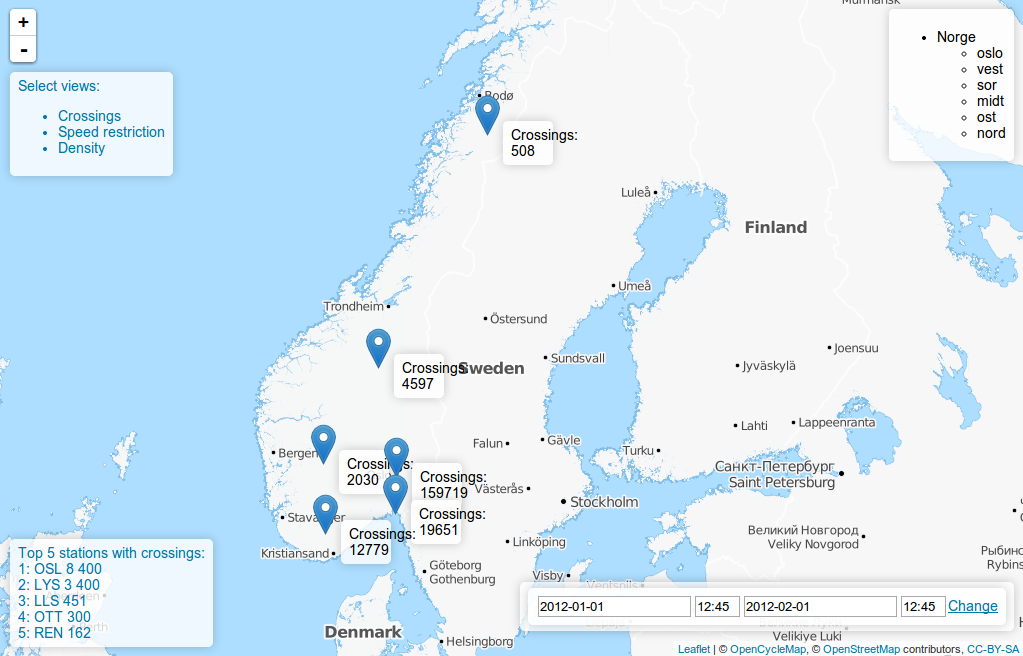
\includegraphics[width=\textwidth,center]{map_prototype.png}
	\caption[Map implementation]{Map implementation}
	\label{fig:map_prototype}
\end{figure}

\begin{figure}[h!tbp]
	\centering
	\begin{subfigure}{0.4\textwidth}
		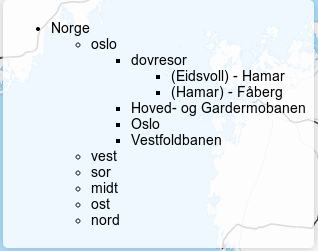
\includegraphics[width=\textwidth]{stakeholder_selection_list.png}
		\caption[Stakeholder selection list]{Stakeholder selection list}
		\label{fig:stakeholder_selection_list}
	\end{subfigure}
	\begin{subfigure}{0.3\textwidth}
		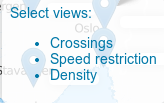
\includegraphics[width=\textwidth]{information_type_selection.png}
		\caption[Information type selection]{Information type selection}
		\label{fig:implementation_type_selection}
	\end{subfigure}
	\caption[Stakeholder selection and Information type]{Stakeholder selection and Information type}
	\label{fig:stakeholder_selection_and_information_type}
\end{figure}

\begin{figure}[h!tbp]
	\centering
	\begin{subfigure}{0.4\textwidth}
		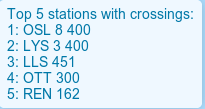
\includegraphics[width=\textwidth]{top5.png}
		\caption[Top 5 list]{Top 5 list}
		\label{fig:top_5_list}
	\end{subfigure}
	\begin{subfigure}{0.6\textwidth}
		
\includegraphics[width=\textwidth]{time_selection_implemented.png}
		\caption[Time selection implementation]{Time selection implementation}
		\label{fig:time_selection_implemented}
	\end{subfigure}
	\caption[Top 5 list and Time selection]{Top 5 list and Time selection}
	\label{fig:Top5_list_and_time_selection}
\end{figure}

\begin{figure}[h!tbp]
	\centering
	\begin{subfigure}{0.6\textwidth}
		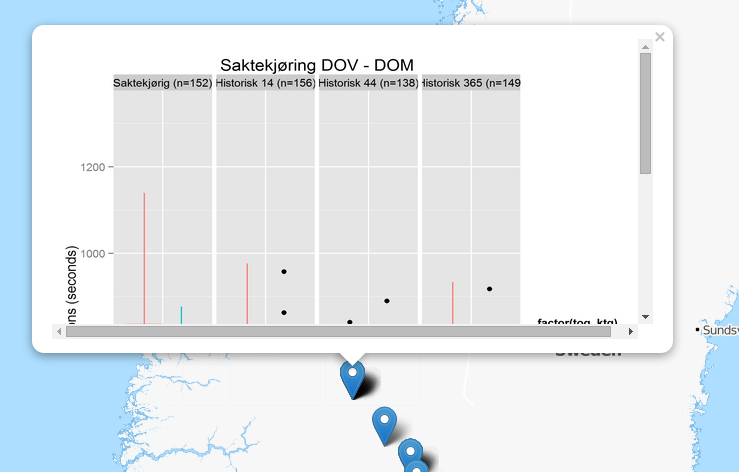
\includegraphics[width=\textwidth]{speed_restriction_presentation.png}
		\caption[Speed restriction presentation]{Speed restriction presentation}
		\label{fig:speed_restriction_presentation}
	\end{subfigure}
	\begin{subfigure}{0.25\textwidth}
		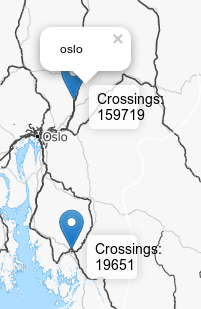
\includegraphics[width=\textwidth]{crossings_presentation.png}
		\caption[Crossings presentation]{Crossings presentation}
		\label{fig:crossings_presentation}
	\end{subfigure}
	\caption[Speed restriction and Crossings implementation]{Speed restriction and Crossings implementation}
	\label{fig:crossings_and_speed_restriction_implementation}
\end{figure}

% section prototype_functionality (end)


% !TEX root=../thesis.tex
\chapter{Discussion}
\label{chapter:discussion}

\section{Stakeholders and aggregation} % (fold)
\label{sec:discussion_stakeholders'_and_aggregation}
It is important to define the needs and requirements of the stakeholders 
early in the process, in order to design a system that gives the right scope. 
By the aid of workshops we defined the requirements, as it is part of the 
research method (see \Ref{sec:workshops}). We can define the stakeholders in 
a hierarchy, based on their organizational structure, and areas of 
responsibility, this aids us in defining the requirements on the structure of 
the information presented.

There is a good synergy between the requirements and the system, when the 
system is designed with the stakeholders' wishes for viewing different type of 
information in mind. The synergy between the requirements and the system has 
both advantages and disadvantages. On one side the system has a great 
possibility to satisfy the requirements and needs of the stakeholders, since 
the system is tightly connected to the requirements. On the other side, the 
system can be inflexible to large changes, if the requirements change late in 
the project. In the workshops, we defined that the stakeholders must have the 
ability to view different kinds of information; the system must take these 
needs into consideration. A system capable of supporting a providing 
“awareness in presentation” of multiple stakeholders is by the very nature 
more complex. Such a system would have to process a larger amount of data than 
a single-perspective system in order to provide the required functionality. 
Processing larger amounts of data leads to a more complex system (back-end) – 
and in turn a more complex interplay between user and front-end, with effects 
on the interplay between front-end and back-end. The system can be more 
dynamic by reusing parts of the data processing for 
different information types, when designed with the needs as well as the 
requirements in mind. In order to meet the requirements of the different 
stakeholders needs we have to aggregate data. There are several ways to 
aggregate the groups of data according to the given criteria. The method used 
for aggregation of data that enables the best view for the stakeholders is not 
straightforward. We have chosen to explore the following simple alternatives: 
average, minimum, maximum, median, and frequency (count). These are by no 
means an exhaustive list, but represent well established, robust and simple to 
implement alternatives. To decide the aggregation method, we have to consider 
how each information type is structured, but also how this structure fits in 
with the stakeholder and their hierarchy. During the workshops, we decided 
that the way to aggregate the data that was best suited to the requirements is 
to take the average; the decision was based on how the data is connected to the stakeholders and their hierarchy.

When returning the processed data to the user, the system can use the 
context of the various stakeholders to aggregate the presentation of the data. Since the stakeholder hierarchy contains the area of responsibility of each stakeholder, the system can fit the visual display to the step of the current stakeholder. The system uses processed data for aggregating the hierarchy to find the stakeholder. Fitting the view to the stakeholder provides detail for a single stakeholder; this is useful for presenting a single stakeholder and their step.
%To let the user decide the detail level of the display can be useful, since the display then has the opportunity to present more overall information. 
We decided to fit the visual presentation of data 
to the current stakeholder, and have the opportunity to jump, back and forth, 
within the hierarchy of the stakeholders. By fitting the view to the 
stakeholder, the display enabled the user to receive more relevant information 
on the current stakeholder. A conflict of interest occurs between stakeholders 
due to overlapping areas of responsibility. The conflict is extremely difficult 
to consider, and is not taken into consideration when aggregating the data or 
fitting the view.

As the area director wants to study data from the entire area for a large 
period of time, and the segment director wants to study almost every detail 
that occurs on the segment, manual navigating in time was decided to use as a 
way to increase and decrease the level of detail in the data presented.

\subsection{Stakeholder and aggreation keywords} % (fold)
\label{sub:stakeholder_and_aggreation_keywords}
Keywords:

\begin{itemize}
	\item Important to define requirements early, in order to make an appropriate system, that is useful for the stakeholders'
	\item How to define the stakeholders' and requirements for use with a system?
	\begin{itemize}
		\item important to define who are the stakeholders'
		\item important to define what the stakeholders' needs are
		\item important to define to which need are connected to which stakeholder, in order to show the correct information in the system connected to each of the stakeholders' needs.
	\end{itemize}
	\item How can we design a system that used the requirements needed by the stakeholders' to process the data and visualize the data in such a way that the stakeholders' needs are met?
	In order to meet the requirements of the stakeholders' needs we need to aggregate the data. The following .....
	\item aggregation of data:
	\begin{itemize}
		\item two goals: geographic \& time
		\item aggregation based on detail level of visualization
		\begin{itemize}
			\item based on stakeholders' need
			\begin{itemize}
				\item detail level in map
				\item which area is shown in the map
				\item aggregation based on time
			\end{itemize}
		\end{itemize}
	\end{itemize}
	\item Data aggregation methods
	\begin{itemize}
		\item What are good ways to aggregate the data?
		\item How to determine what fits the requirements?
	\end{itemize}
	\item How to present the data to the users based on the requirements? (detail
	level per stakeholder in the hierarchy)
	\item Time navigation for zooming through the data.
\end{itemize}

% subsection stakeholder_and_aggreation_keywords (end)


% section stakeholders'_and_aggregation (end)

\section{Data storage and data queries} % (fold)
\label{sec:discussion_data_storage_and_data_queries}
As the data sets originate from different sources and contain different
structures, they can be difficult to efficiently query if not structured
correctly. One option for the structure is to merge all the
data sets into one large database, by merging the data sets in one large
database, the data are structured in an client-server architecture. 
A client can either communicate to the databases directly or through a middle
tier. Three-tier architecture is a very common solution on the Internet, where 
the communication between the client and the database goes through a service 
layer \cite[pp. 294-297]{toftHanseMallaugDatabaser}. The client-server 
architecture has the benefits of giving the front-end applications a single 
point of connection, avoiding duplication of data, and giving the database 
manager both a single structure to maintain and a single point of access with 
easier access control.

The alternative of the client-server architecture is a distributed
database \cite[pp. 301-303]{toftHanseMallaugDatabaser}. The distributed database
architecture is done by splitting the storage of data and the processing of
data over several servers. Some benefits of the distributed architecture are 
easier expansion, modular sets with built-inn flexibility, and if one node 
goes down the others still work. Exercising the built-inn flexibility of each
module is usually cheaper than to hand-code a specific change in hindsight\cite[pp. 117-130]{Bass:2012:SAP:2392670}. The distributed architecture is a 
modifiable data storage, where the modular sets are loosely linked sets. 
%software architecture p. 185 for other quality attributes
We demonstrated a hybrid of the client-server and distributed
architecture \cite[pp. 297-299]{toftHanseMallaugDatabaser}.

By using the three-tier architecture, we implemented a middle-tier which 
processed the data, and a lower tier containing several databases, see \Ref{fig:three-tier_architecture}. For
structuring the data sets with the stakeholders' requirements in mind, we
utilized one database which contained the stakeholders' areas of responsibility in
their hierarchy, and each of the other databases for different types of 
information. The semi-distributed databases mean that it is easy to remove or
add data sets, since the different types of information are connected to the
stakeholders' hierarchy. There are also some negative aspects using
the semi-distributed databases, for example: some data fields
will be duplicated. The duplication of data will lead to redundancy and
increased probability for data corruption and errors. In our case the duplication can be found as stations in the databases, due to the stations acting as the
connection between every data set. In the three-tier, distributed database, 
and semi-distributed architecture, the data have to be processed from the 
original source to fit in with the data structure.\\

We can increase the responsiveness of the system by utilizing the back-end for 
processing the data, since it usually on the same hardware as the databases or 
same sub-net, which provides quicker calls and responses to the databases from 
the data processing methods. As the aggregation averages the data based on the variables selected by the user, the data transferred from the back-end to the front-end will be reduced. Having a reduced amount of data to transfer, means that the system will experience quicker communication times. We 
have no control over what hardware the end user has, while the back-end 
is usually dedicated to one service and we can (more easily) control, and if 
necessary upgrade, the hardware.

The amount of data to be processed by the system is affected by three 
variables. The affecting variables are the stakeholders' need to navigate in 
time, the navigating in the stakeholder hierarchy, and the type of information.
As the level of detail increases by navigating in time, the amount of data to 
process decreases. Similarly by decreasing the level of detail, the amount of 
data to process increases. The navigation in the hierarchy affects the amount 
of data, as the further up in the hierarchy one navigates, the larger the 
areas of responsibility grows. The information type affects the amount of data 
in a data-set, because each information type have different needs for the 
amount of data to be processed. The system performance is determined by the 
amount of data to process, as it uses more time to process more data. 

\subsection{Data storage and data queries keywords} % (fold)
\label{sub:data_storage_and_data_queries_keywords}
Keywords:
\begin{itemize}
	\item Data set structure in prototype
	\begin{itemize}
		\item How should the data sets be structured when the sets are based 
		on the stakeholders' need for different type of information?
		\begin{itemize}
			\item Connection to the requirements of the stakeholders'.
			\begin{itemize}
				\item Stakeholder responsibility area from the hierarchy
			\end{itemize}
			\item Advantages and disadvantages with one or several sets in storage.
			\begin{itemize}
				\item Scalability and modifiability ref quality attributes \cite{Bass:2012:SAP:2392670}
				\item Duplication of data with several sets of data.
			\end{itemize}
		\end{itemize}
	\end{itemize}
	\item Data queries
	\begin{itemize}
		\item Limit queries for data processing efficiency 
		and more responsive systems
		\begin{itemize}
			\item By the aid of time navigation and requirements, limit the 
			queries for more efficient calls to the data storage.
			\item The system will be more efficient in the processing of the 
			data, when limiting the quires.
		\end{itemize}
		\item Front end vs back end data processing for system efficiency and
		limiting data traffic
		\item Should the data be processed in the front-end or the back-end 
		of the system?
		\begin{itemize}
			\item The data should be aggregated in the back-end of the system, 
			since it is more efficient.
			\begin{itemize}
				\item Quicker calls to the database from the back-end.
				\item Less data traffic during transfer of.
				\item Usually quick hardware on server side, while it have a 
				great span in the front-end.
			\end{itemize}
		\end{itemize}
	\end{itemize}
\end{itemize}

% subsection data_storage_and_data_queries_keywords (end)

% section data_storage_and_queries (end)

%\section{Review of own work} % (fold)
%\label{sec:review_of_own_work}
%Keywords:
%\begin{itemize}
%	\item Appropriate method?
%	\item 
%\end{itemize}
% section review_of_own_work (end)

% !TEX root=../thesis.tex
\chapter{Conclusion and future work}
\label{chapter:conclusion}


\cleardoublepage
\renewcommand\bibname{References}
\phantomsection
\addcontentsline{toc}{chapter}{\bibname}
\label{bibliography}
\bibliography{bibliography}
%\nocite{*} %All
%\nocite{key1,key2,keyN}

%Use ieeetr to get correct numbering of references according to the IEEE
% standard. Numbering follows order of introduction.
\bibliographystyle{ieeetr}

\end{document}
